\documentclass[a4paper,12pt]{article}
\usepackage{imakeidx}
\usepackage{graphicx}
\usepackage{float} %required for the placement specifier H
\usepackage{multicol}		%multicolumns
\usepackage{tabto}
\usepackage{listings}
\usepackage{comment}
\UseRawInputEncoding
\usepackage{fancyvrb}

\usepackage{color}
\usepackage[a4paper,colorlinks=true,urlcolor=blue,citecolor=blue,linkcolor=blue,bookmarks=false]{hyperref}
\usepackage{xspace}
% Definition of margins
%
\usepackage[top=2cm,bottom=2cm,left=2cm,right=2cm]{geometry}

\definecolor{dkgreen}{rgb}{0,0.6,0}
\definecolor{gray}{rgb}{0.5,0.5,0.5}
\definecolor{mauve}{rgb}{0.58,0,0.82}

\lstset{frame=tb,
  language=c,
  aboveskip=3mm,
  belowskip=3mm,
  showstringspaces=false,
  columns=flexible,
  basicstyle={\small\ttfamily},
  numbers=none,
  numberstyle=\tiny\color{gray},
  keywordstyle=\color{blue},
  commentstyle=\color{dkgreen},
  stringstyle=\color{mauve},
  breaklines=true,
  breakatwhitespace=true,
  tabsize=3
}

\usepackage[english]{babel}
\usepackage[latin1]{inputenc}% IMPORTANT! use ISO-8859-1 encoding
\usepackage{xcolor}
\usepackage{adjustbox}
\usepackage{verbatim}
\definecolor{shadecolor}{rgb}{.10, .10, .10}

\makeindex[columns=3]



\setlength\parskip{\medskipamount}
\setlength\parindent{0pt}

\begin{document}

%opening
\title{WolfSSL
\\
{\normalsize Report for the Information System Security exam at the Politecnico di Torino}
}
\author{Luca Valentini (278487)
\\
}
\date{december 2020}
\maketitle
\vfill

\rule{\textwidth}{1pt}

\tableofcontents

\rule{\textwidth}{1pt}

\vfill


\newpage
\begin{abstract}
This document was intended as a small introductory guide to wolfssl.
For the creation of this thesis I used the official wolfssl manual and some github repository related to wolfssl.
\end{abstract}
\newpage


\section{Communication Security In Embedded Systems}
\textit{An embedded system can be defined as an autonomous electronic and information system} \cite{BookEmbeddedSystems}.
An embedded system is not really a personal computer (PC), but may resemble an industrial PC.  We can see that a standard PC can execute all types of applications as it is designed for general purposes, while an embedded system can only execute a single dedicated application
An important property of an embedded system is its ability to communicate with the outside world. The processors used in an embedded system integrate an Ethernet network interface as standard. It is also possible to integrate a wired or wireless internet connection simply by the addition of a small electronic module. Today, controlling an embedded system from a distance has become a reality, and it is completely possible to control an embedded system over the internet via a web browser. This is possible thanks to the power offered by processors designed for embedded systems, and also to the explosion in internet connectivity and the way in which this has become a part of everyday life. IP connectivity basically allows us to control an embedded system remotely over the internet.

Nevertheless, an important problem emerges: communications security in embedded systems in the current situation.
With the growing number of embedded applications (aircraft or factory control, transactions, video, etc.), various embedded systems have to communicate with each other over non-secure channels, such as the internet, via wireless connections. There is therefore an enormous risk if data, commands, or sensitive updates are transmitted insecurely over the internet. In order to withstand malicious attacks, the data exchanged must be secured from one end of the transmission to the other. Today many protocols for securing communications (SSH, SSL/TLS, DTLS, IPsec, etc.) are available, and security can be implemented at various levels of the communication stack. However, the greatest obstacles to their use in embedded systems are the limited memory and low processing capacity provided by the platforms of these devices.

Cryptographic algorithms with their many calculations and their significant demands on memory have always presented a barrier to the addition of security to communications among embedded systems. Today, these barriers have become less and less important thanks to the adaptation of security protocols for embedded systems and the use of hardware acceleration techniques, which provide low power processors with the capacity to rapidly execute cryptographic algorithms.

\section{WolfSSL}
\subsection{Introduction}

The wolfSSL embedded library is a lightweight TLS library written in ANSI C and targeted for embedded, RTOS, and resource-constrained
environments - primarily because of its small size, speed, and feature set; It's an SSL/TLS library optimized to run on embedded platforms.
It's free and it has an excellent cross platform support.

WolfSSL supports SSL 3.0, TLS(1.0, 1.1, 1.2, 1.3), and DTLS(1.0, 1.2).
It also includes an OpenSSL compatibility interface with the most commonly used OpenSSL functions.
WolfSSL is open source, licensed under the GNU General Public License GPLv2.

%\vspace{5mm} %5mm vertical space
This library is built for maximum portability and supports the C programming language as a primary interface. It also supports several other host languages, including Java (wolfSSL JNI), C\# (wolfSSL C\#), Python, and PHP and Perl.

%\vspace{5mm} %5mm vertical space
To improve performance it supports hardware cryptography and acceleration on several platforms.

%\vspace{5mm} %5mm vertical space
WolfSSL uses the following cryptography libraries:
\begin{itemize}
\item wolfCrypt
\begin{itemize}
\item Provides RSA, ECC, DSS, Diffie?Hellman, EDH, NTRU, DES, Triple DES, AES (CBC, CTR, CCM, GCM), Camellia, IDEA, ARC4, HC-128, ChaCha20, MD2, MD4, MD5, SHA-1, SHA-2, SHA-3, BLAKE2, RIPEMD-160, Poly1305, Random Number Generation, Large Integer support, and base 16/64 encoding/decoding.
\end{itemize}
\item NTRU
\begin{itemize}
\item An open source public-key cryptosystem that uses lattice-based cryptography to encrypt and decrypt data. 
\end{itemize}
\end{itemize}

\cleardoublepage
\subsection{Operating system supported}

The operating systems supported are:
\begin{multicols}{3}
\begin{enumerate}
\item Win32/64 \item Linux \item Mac OS X \item Solaris \item ThreadX \item VxWorks \item FreeBSD \item NetBSD \item OpenBSD \item embedded Linux \item Yocto Linux \item OpenEmbedded \item WinCE \item Haiku \item OpenWRT \item iPhone(iOS) \item Android \item Nintendo Wii and Gamecube through DevKitPro \item QNX \item MontaVista \item NonStop \item TRON / ITRON /  ITRON \item Micrium  C / OS - III \item FreeRTOS \item SafeRTOS \item NXP / Freescale MQX \item Nucleus \item TinyOS \item HP / UX \item AIX \item ARC MQX \item TI - RTOS \item uTasker \item embOS \item INtime \item Mbed \item uT - Kernel \item RIOT \item CMSIS -RTOS \item FROSTED \item Green Hills INTEGRITY \item Keil RTX \item TOPPERS \item PetaLinux \item Apache Mynewt \item PikeOS 
\end{enumerate}
\end{multicols}
\cleardoublepage
\subsection{WolfSSL's features}
\begin{itemize}
\item Runtime memory usage between 1-36 kB
\item Minimum footprint size of 20-100 kB, depending on build options and operating environment
\item OpenSSl compatibility layer
\item Hash Functions: \begin{multicols}{3}\begin{itemize}
\item MD2
\item MD4
\item MD5
\item SHA-1
\item SHA-224
\item SHA-256
\item SHA-384
\item SHA-512
\item BLAKE2b
\item RIPEMD-160
\item Poly1305
\end{itemize}
\end{multicols}
\item OCSP, OCSP Stapling, and CRL support
\item Block, Stream, and Authenticated Ciphers:
\begin{itemize}
\item AES (CBC, CTR, GCM, CCM, GMAC, CMAC), Camellia, DES, 3DES, IDEA, ARC4, RABBIT, HC-128, ChaCha20
\end{itemize}
\item Public Key Algorithms:
\begin{itemize}
\item RSA, DSS, DH, EDH, ECDH-ECDSA, ECDHE-ECDSA, ECDH-RSA, ECDHE-RSA, NTRU
\end{itemize}
\item Password-based Key Derivation: HMAC, PBKDF2
\item Curve25519 and Ed25519
\item ECC and RSA Key Generation
\item X.509v3 RSA and ECC Signed Certificate Generation
\item PEM and DER certificate support
\item Modular cryptography library (wolfCrypt)
\item Open Source Project Integrations:
\begin{itemize}
\item MySQL, OpenSSH, Apache httpd, Open vSwitch, stunnel, Lighttpd, GoAhead, Mongoose, and more!
\end{itemize}
\item PKCS\#1 (RSA Cryptography Standard) support
\item PKCS\#3 (Diffie-Hellman Key Agreement Standard) support
\item PKCS\#5 (Password-Based Encryption Standard) support
\item PKCS\#7 (Cryptographic Message Syntax - CMS) support
\item PKCS\#8 (Private-Key Information Syntax Standard) support
\item PKCS\#9 (Selected Attribute Types) support
\item PKCS\#10 (Certificate Signing Request - CSR) support
\item PKCS\#11 (Cryptographic Token Interface) support
\item PKCS\#12 (Certificate/Personal Information Exchange Syntax Standard) support
\item Mutual authentication support (client/server)
\item SSL Sniffer (SSL Inspection) Support
\item IPv4 and IPv6 support
\end{itemize}


\section{Test case}
\subsection{Client/Server provided by WolSSL}

\begin{figure}[H]
\begin{Verbatim}[commandchars=\\\{\}]
______________________________________________________________
\textcolor{green}{pi@raspberrypi}\textcolor{black}{:}\textcolor{blue}{wolfSSL/wolfssl/examples/server}\textcolor{black}{$ ./server -b}
SSL VERSION is TLSv1.2
SSL ciphet suite is TLS_ECDHE_RASA_WITH_AES_256_GCM_SHA384
SSL curve name is SECP256R1
Client message: hello wolfssl!
______________________________________________________________
\end{Verbatim}
\caption{Server TLS}
\end{figure}

\begin{figure}[H]
\begin{Verbatim}[commandchars=\\\{\}]
______________________________________________________________
\textcolor{green}{luca@luca}\textcolor{black}{:}\textcolor{blue}{wolfSSL/wolfssl/examples/client}\textcolor{black}{$ ./client -h }
192.168.0.53
SSL VERSION is TLSv1.2
SSL ciphet suite is TLS_ECDHE_RASA_WITH_AES_256_GCM_SHA384
SSL curve name is SECP256R1
I hear you fa shizzle!
______________________________________________________________
\end{Verbatim}
\caption{Client TLS}
\end{figure}


In this example, the server is a simple TLS server that allows only one client connection; after the connection with a client, the server receives an encrypted message from client, it responds and quits.
The -b parameter allows the server to bind to any interface instead of localhost only.

After the connection with the server, the client sends a message (hello wolfssl!) and, after the server response, the client quits.
The -h parameter allows the client to specify the server address to perform the connection.

\begin{figure}[H]
    \centering
    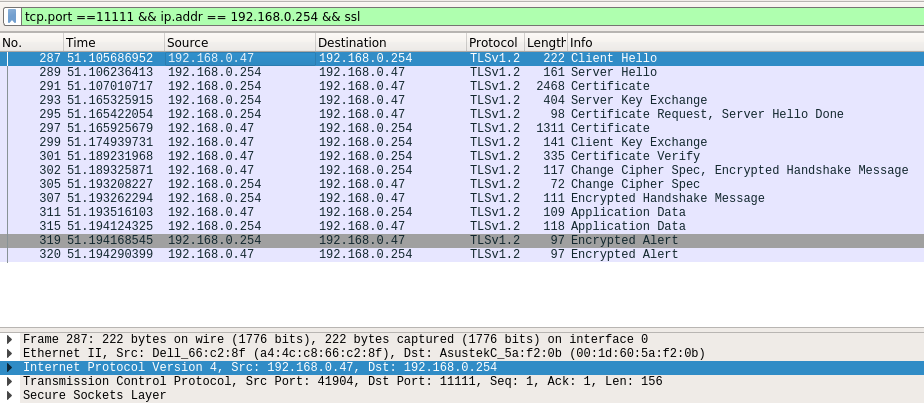
\includegraphics[scale=0.22]{test/examples/client-server/wireshark1.png}
    \caption{All TLS packets sent}
    
\end{figure}
Client IP:  192.168.0.47 \hspace{4cm} Server IP: 192.168.0.53\\ \\
As you can see from the figure above, the communication is initialized from client with a 'Client Hello'; after TLS handshake, there are 2 messages 'Application Data' sent respectively from the client to the server and from the server to the client, whose content is encrypted. Once the server sends a response to the client, the communication is closed.

\begin{figure}[H]
    \centering
    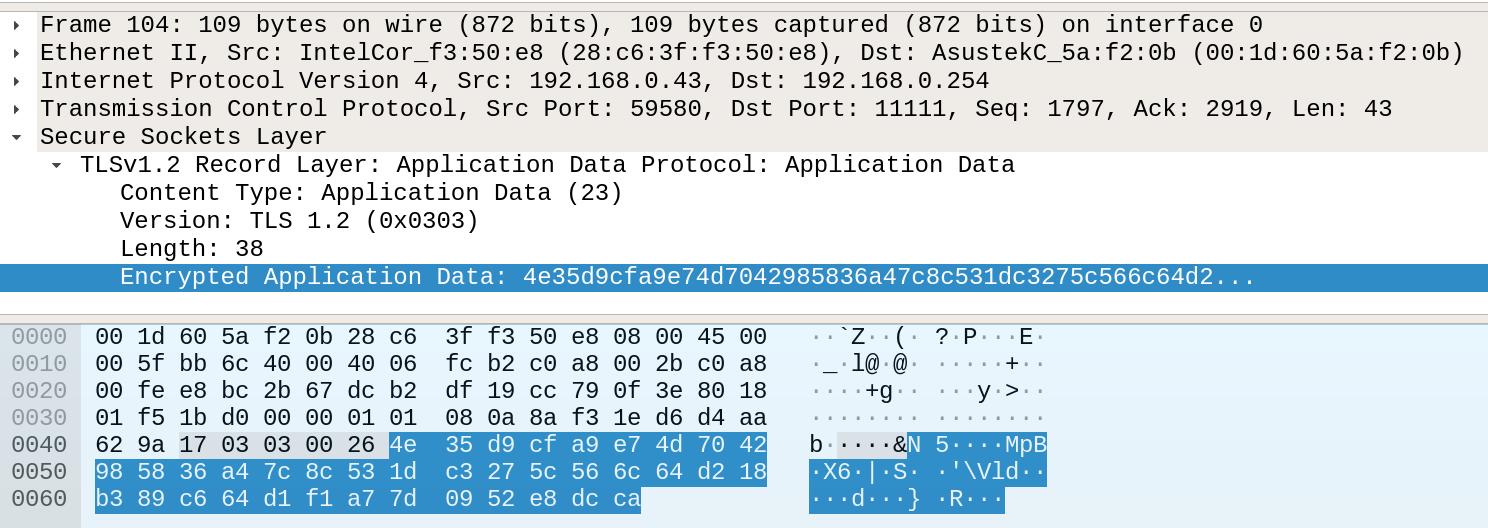
\includegraphics[scale=0.27]{test/examples/client-server/encrypted_data.png}
    \caption{Content of the encrypted message}
    
\end{figure}


\begin{comment}
\subsection{EchoClient/EchoServer provided by WolfSSL}
\begin{figure}[H]
\hspace*{-1cm}     
    \centering
    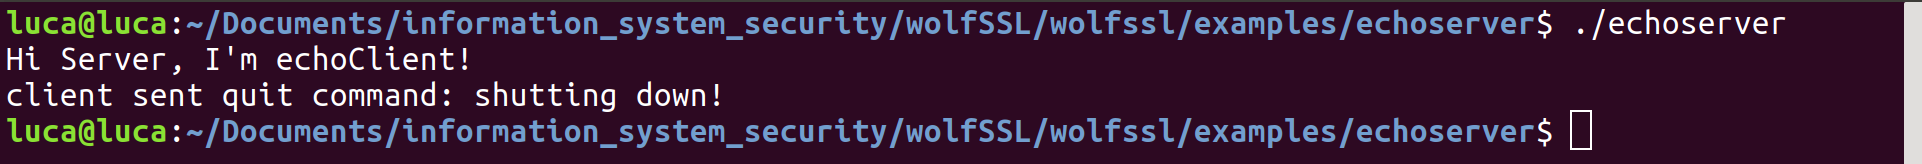
\includegraphics[scale=0.25]{test/examples/echoclient-echoserver/echoServer.png}
    \caption{EchoServer TLS}
    
\end{figure}

\begin{figure}[H]
\hspace*{-1cm}     
    \centering
    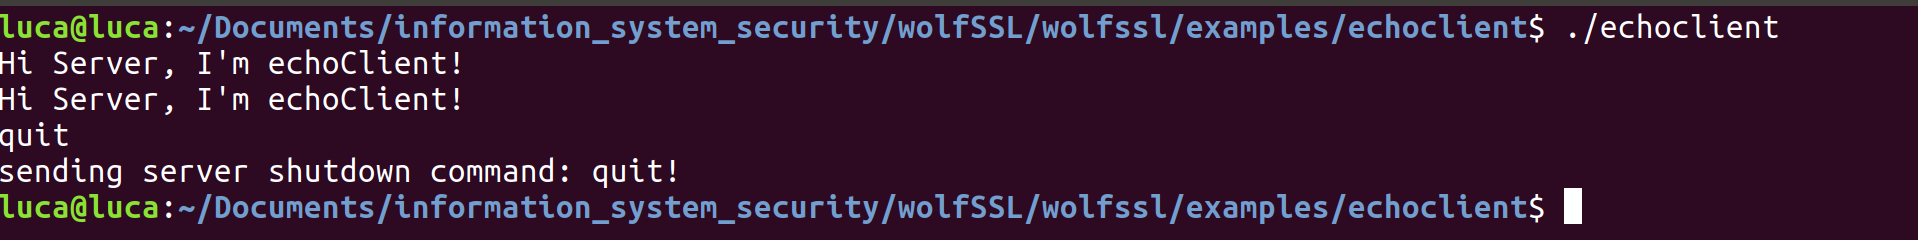
\includegraphics[scale=0.25]{test/examples/echoclient-echoserver/echoClient.png}
    \caption{EchoClient TLS}
    
\end{figure}

\begin{figure}[H]
\hspace*{-2cm}     
    \centering
    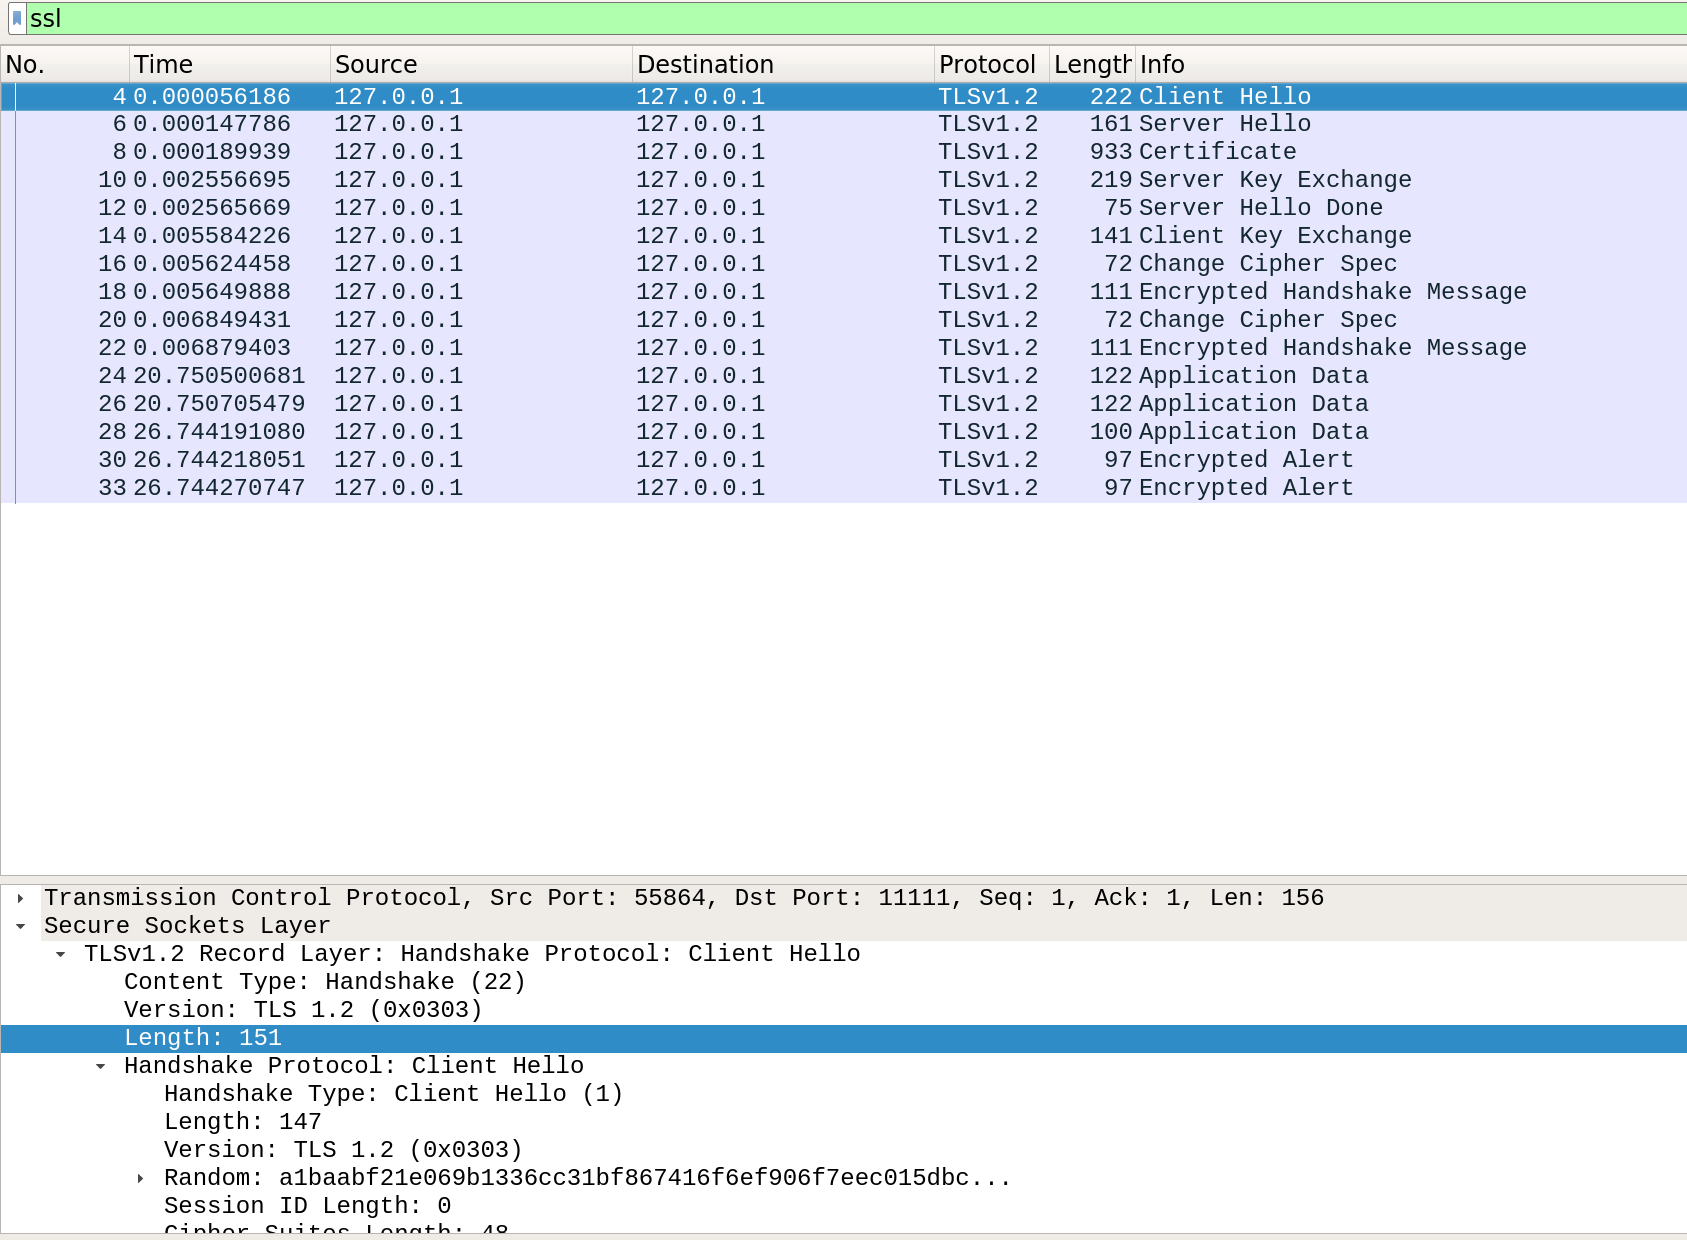
\includegraphics[scale=0.3]{test/examples/echoclient-echoserver/wireshark.png}
    \caption{All TLS packets sent}
    
\end{figure}
\end{comment}

\section{Create a program using WolfSSL}
\subsection{TCP application}
To create a TLS program you can modify your TCP program by adding several TLS functions. To explain the migration from TCP to TLS, I created a simple chat between a client and a server. The code of this program isn't reported in this text but it is available on github.

%\vspace{5mm} %5mm vertical space
In the picture there is a wireshark screenshot to see the data traffic of a tcp application; this image with the next sections allows to understand the difference between an application with or without encryption.

\begin{figure}[H]
    \centering
    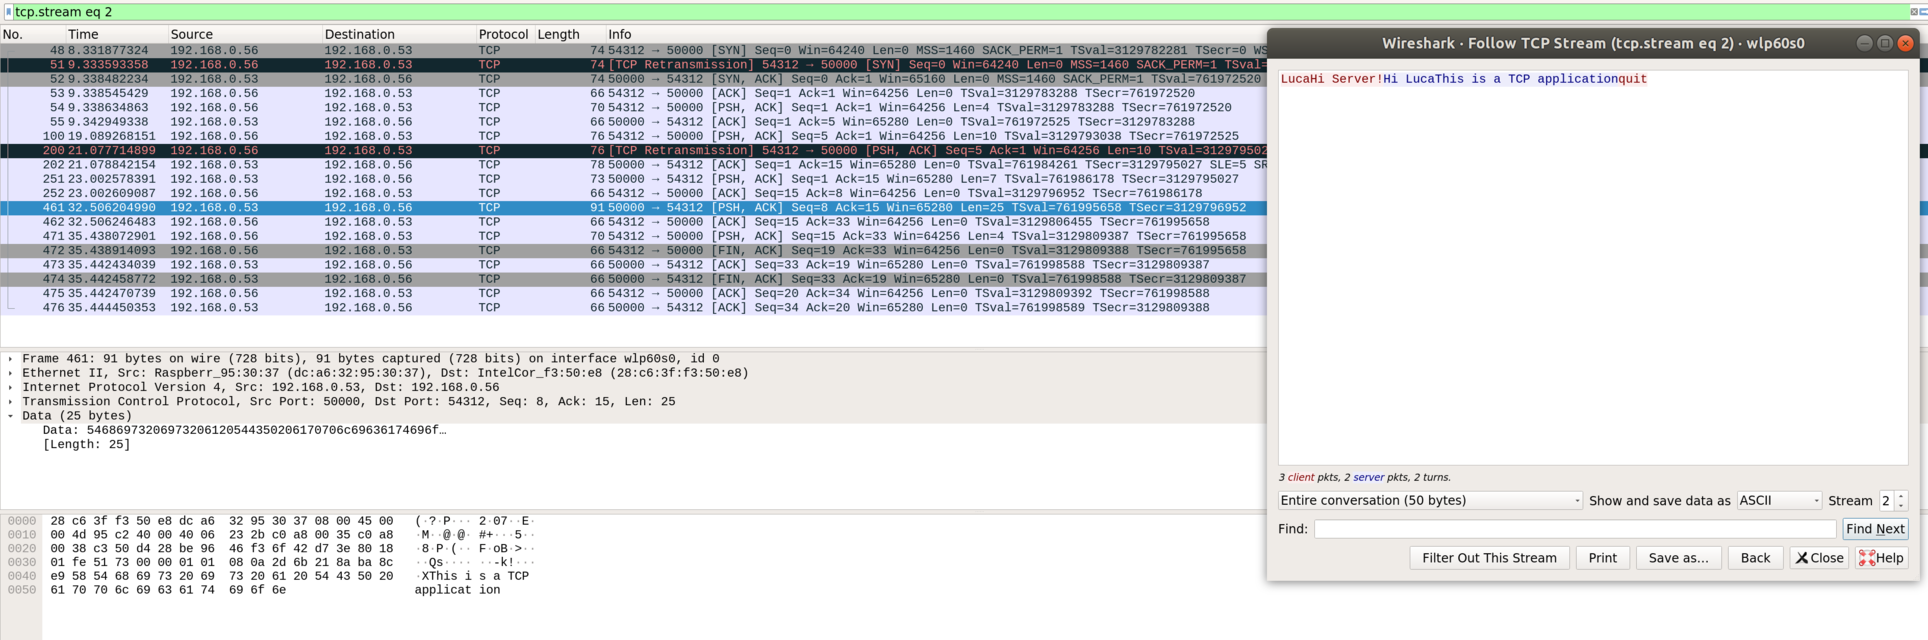
\includegraphics[scale=0.23]{./code/tcp/img/test.png}
    \caption{TCP data traffic}
    
\end{figure}



\begin{comment}
\subsection{TCP Server}

In my example, the TCP server after configuring the socket and connecting it with the client, it creates a ClientHandler thread that launches a thread for read and a thread for write from socket.
\begin{lstlisting}[caption={int main() of TCP server},captionpos=b][language=c]

int main()
{
    /* Create a socket that uses an internet IPv4 address,
     * Sets the socket to be stream based (TCP),
     * 0 means choose the default protocol. */
    if ((sockfd = socket(AF_INET, SOCK_STREAM, 0)) == -1)
    {
        fprintf(stderr, "ERROR: failed to create the socket\n");
        return -1;
    }

    /* Initialize the server address struct with zeros */
    memset(&servAddr, 0, sizeof(servAddr));

    /* Fill in the server address */
    servAddr.sin_family = AF_INET;           /* using IPv4      */
    servAddr.sin_port = htons(DEFAULT_PORT); /* on DEFAULT_PORT */
    servAddr.sin_addr.s_addr = INADDR_ANY;   /* from anywhere   */

    /* Bind the server socket to our port */
    if (bind(sockfd, (struct sockaddr *)&servAddr, sizeof(servAddr)) == -1)
    {
        fprintf(stderr, "ERROR: failed to bind\n");
        return -1;
    }

    /* Listen for a new connection*/
    if (listen(sockfd, 1) == -1)
    {
        fprintf(stderr, "ERROR: failed to listen\n");
        return -1;
    }
    /* Continue to accept clients until shutdown is issued */
    while (1)
    {
        printf("Waiting for a connection...\n");
        /* Accept client connections */
        if ((connd = accept(sockfd, (struct sockaddr *)&clientAddr, &size)) == -1)
        {
            fprintf(stderr, "ERROR: failed to accept the connection\n\n");
            ncurses_end();
            return -1;
        }
        pthread_t mainThread;
        pthread_create(&mainThread, NULL, ClientHandler, NULL);
        pthread_join(mainThread, NULL);
        printText("Communication is ended!\n", "System");

        if (is_end)
            break;
    }
    ncurses_end();
    printf("Shutdown complete\n");

    /* Cleanup after this connection */
    close(connd); /* Close the connection to the client   */
    /* Cleanup and return */
    close(sockfd); /* Close the socket listening for clients   */
    return 0;      /* Return reporting a success               */
}

\end{lstlisting}

As stated above, the clientHandler thread creates two thread, but before it waits the client username.

\begin{lstlisting}[caption={clientHandler thread of TCP server},captionpos=b][language=c]
void *ClientHandler(void *args)
{
    int ret;
    /*********************** USERNAME */
    /* Read the client username into our buff array */
    XMEMSET(buff, 0, sizeof(buff));
    ret = read(connd, buff, sizeof(buff));
    ncurses_start();
    clearWin();
    if (ret > 0)
    {
        /* Print to stdout any data the client sends */
        strcpy(username, buff);
        char text[256];
        sprintf(text, "Client %s connected successfully", username);
        printText(text, "System");
        printText("***************************\n", "System");
        fflush(stdout);
    }
    else
    {
        printText("ERROR!!", "System");
        close(sockfd);      /* Close the connection to the server   */
        pthread_exit(NULL); /* End threaded execution                */
    }
    /****************************    */
    XMEMSET(buff, 0, sizeof(buff));

    if (pthread_create(&Treader, NULL, readBuffer, NULL))
    {
        fprintf(stderr, "Error creating thread\n");
        fflush(stdout);
        return NULL;
    }

    if (pthread_create(&Twriter, NULL, writeBuffer, NULL))
    {
        fprintf(stderr, "Error creating thread\n");
        fflush(stdout);
        return NULL;
    }
    pthread_join(Treader, NULL);
    pthread_join(Twriter, NULL);
    /* Cleanup after this connection */
    close(connd);       /* Close the connection to the client   */
    pthread_exit(NULL); /* End threaded execution                */
}

\end{lstlisting}


ReadBuffer is a thread that allows to read messages sent from client. It has an infinite loop that read data from socket open previously; Once it gets the message, with the printText function, the message is printed to the terminal using ncurses. 
\begin{lstlisting}[caption={readBuffer thread of TCP server},captionpos=b][language=c]
void *readBuffer(void *args)
{
    int ret;
    while (1)
    {
        /* Read the client data into our buff array */
        XMEMSET(buffReader, 0, sizeof(buffReader));
        ret = read(connd, buffReader, sizeof(buffReader));

        if (ret > 0)
        {
            if (!strcmp(buffReader, "quit"))
            {
                pthread_cancel(Twriter);
                pthread_exit(NULL); /* End threaded execution                */
            }
            printText(buffReader, username);
        }
        else
        {
            printText("ERROR READ!!", "System");
            pthread_cancel(Twriter);
            pthread_exit(NULL); /* End threaded execution                */
        }
    }
}

\end{lstlisting}
WriteBuffer thread has an infinite loop used for write messages from server to client.
\begin{lstlisting}[caption={writeBuffer thread of TCP server},captionpos=b][language=c]
void *writeBuffer(void *args)
{
    int ret;
    while (1)
    {
        read_in();
        len = XSTRLEN(Rbuffer);

        /* Reply back to the client */
        ret = write(connd, Rbuffer, len);
        printText(Rbuffer, "Server");

        if (XSTRNCMP(Rbuffer, "quit", 4) == 0)
        {
            is_end = 1;
            break;
        }

        if (ret != len)
        {
            printText("ERROR!!", "System");
            break;
        }
    }
    pthread_cancel(Treader);
    return NULL;
}

\end{lstlisting}
\end{comment}
\subsection{From TCP to TLS}
To create a wolfSSL application the first thing that I did was including the wolfSSL API header in my program.
\begin{lstlisting}[language=c]
#include <wolfssl/ssl.h>
\end{lstlisting}
After the inclusion of the header files, I initialized the library and the WOLFSSL\_CTX calling \textbf{wolfSSL\_Init}; it is necessary to use the library.

The WOLFSSL\_CTX structure contains global values for each SSL connection, including certificate information.
To create a new WOLFSSL\_CTX there is \textbf{wolfSSL\_CTX\_new()} function. It requires an argument which defines the SSL or TLS protocol for the client or server to use. In my case I used TLS 1.3, so the call is: 
\begin{lstlisting}[language=c]
WOLFSSL_CTX *ctx = wolfSSL_CTX_new(wolfTLSv1_3_server_method());
\end{lstlisting}
for the server;
\begin{lstlisting}[language=c]
WOLFSSL_CTX *ctx = wolfSSL_CTX_new(wolfTLSv1_3_client_method())
\end{lstlisting}
for the client.

In the WOLFSSL\_CTX the CA (Certificate Authority) can be loaded so that the client is able to verify the server's identity when they start the connection. To load the CA into the WOLFSSL\_CTX there is \\\textbf{wolfSSL\_CTX\_load\_verify\_locations()}. This function requires three arguments:
\begin{itemize}
\item a WOLFSSL\_CTX pointer
\item a certificate file
\item a path value that point to a directory which should contain CA certificates in PEM format.
\end{itemize}
this function returns SSL\_SUCCESS or SSL\_FAILURE.

\textbf{wolfSSL\_CTX\_load\_verify\_locations()} can be used to verify the certificate of the servers by the client.
The server loads a certificate file into the TLS context (WOLFSSL\_CTX) through this function:
\begin{lstlisting}[language=c]
int wolfSSL_CTX_use_certificate_file(ctx, CERT_FILE, SSL_FILETYPE_PEM);
\end{lstlisting}
Then the server must load the private key with:
\begin{lstlisting}[language=c]
int wolfSSL_CTX_use_PrivateKey_file(ctx, KEY_FILE, SSL_FILETYPE_PEM)
\end{lstlisting}

After a TCP connection the WOLFSSL object needs to be created and the file descriptor needs to be associated with the session; the instructions are:
\begin{lstlisting}[language=c]
//Connect to socket file descriptor
WOLFSSL* ssl;
//create WOLFSSL object
ssl = wolfSSL_new(ctx);
wolfSSL_set_fd(ssl,sockfd);
\end{lstlisting}
After the previous instructions called by client and server, the server waits for a TLS client to initiate the SSL handshake; it waits until a client calls \textbf{wolfSSL\_connect(ssl)} and then the handshake starts.

Once the connection functions were set, I replaced \textbf{read(...)} function with: 
\begin{lstlisting}[language=c]
int wolfSSL_read(WOLFSSL *ssl, void *data, int sz);
\end{lstlisting}
It read \textbf{sz} bytes from the SSL session \textbf{ssl} internal read buffer into the buffer \textbf{data}. The bytes are removed from the internal receive buffer;

Instead the \textbf{write(...)} function is replaced by:
\begin{lstlisting}[language=c]
int wolfSSL_write(WOLFSSL *ssl, void *data, int sz);
\end{lstlisting}
It writes \textbf{sz} bytes from the buffer, \textbf{data}, to the TLS connection, \textbf{ssl}.

When the application is over, the WOLFSSL\_CTX object and the wolfSSL library must be freed; the instructions are:
\begin{lstlisting}[language=c]
wolfSSL_free(ssl);
wolfSSL_CTX_free(ctx);
wolfSSL_Cleanup();
\end{lstlisting}


\subsection{TLS programs}
To develop a TLS application, I started from the TCP chat explained in the previous subsection and I added the wolfSSL function to create an encrypted communication.
Next programmes' aim is to show how to create a simple encrypted chat, focusing on the security of applications, rather than on the good practices of the socket and thread applications.
Some parts of the code like inclusion and global variables are omitted (wolfSSL object and other variables are stored in global memory); 
\subsubsection{Iterative program}
In the next sections I'll try to explain the code of programs created by me:
the iterative wolfSSL program is a very simple chat between two host, a client and a server; it's a ping pong chat where a client can write only if the server write first.
For testing purpose, all the certificates that I use and the server private key were taken from wolfSSL download.
After the initialization of the wolfSSL and the socket, the main function marks the socket referred to by sockfd as a passive socket, that is, as a socket that will be used to accept an incoming connection request using accept.
\begin{lstlisting}[caption={int main() of iterative TLS server},captionpos=b][language=c]
int main()
{
    int ret;

    /* Initialize wolfSSL */
    wolfSSL_Init();

    /* Create a socket that uses an internet IPv4 address,
     * Sets the socket to be stream based (TCP),
     * 0 means choose the default protocol. */
    if ((sockfd = socket(AF_INET, SOCK_STREAM, 0)) == -1)
    {
        fprintf(stderr, "ERROR: failed to create the socket\n");
        return -1;
    }
    if (setsockopt(sockfd, SOL_SOCKET, SO_REUSEADDR, &(int){1}, sizeof(int)) < 0)
    {
        printf("setsockopt(SO_REUSEADDR) failed");
        return -1;
    }

    /* Create and initialize WOLFSSL_CTX */

    if ((ctx = wolfSSL_CTX_new(wolfTLSv1_2_server_method())) == NULL)
    {
        fprintf(stderr, "ERROR: failed to create WOLFSSL_CTX\n");
        return -1;
    }

    /* Load server certificates into WOLFSSL_CTX */
    if (wolfSSL_CTX_use_certificate_file(ctx, CERT_FILE, SSL_FILETYPE_PEM) != SSL_SUCCESS)
    {
        fprintf(stderr, "ERROR: failed to load %s, please check the file.\n",
                CERT_FILE);
        return -1;
    }

    /* Load server key into WOLFSSL_CTX */
    if (wolfSSL_CTX_use_PrivateKey_file(ctx, KEY_FILE, SSL_FILETYPE_PEM) != SSL_SUCCESS)
    {
        fprintf(stderr, "ERROR: failed to load %s, please check the file.\n",
                KEY_FILE);
        return -1;
    }

    /* Initialize the server address struct with zeros */
    memset(&servAddr, 0, sizeof(servAddr));

    /* Fill in the server address */
    servAddr.sin_family = AF_INET;           /* using IPv4      */
    servAddr.sin_port = htons(DEFAULT_PORT); /* on DEFAULT_PORT */
    servAddr.sin_addr.s_addr = INADDR_ANY;   /* from anywhere   */

    /* Bind the server socket to our port */
    if (bind(sockfd, (struct sockaddr *)&servAddr, sizeof(servAddr)) == -1)
    {
        fprintf(stderr, "ERROR: failed to bind\n");
        return -1;
    }

    /* Listen for a new connection */
    if (listen(sockfd, 1) == -1)
    {
        fprintf(stderr, "ERROR: failed to listen\n");
        return -1;
    }
    printf("Waiting for a connection...\n");
    /* Accept client connections */
    if ((connd = accept(sockfd, (struct sockaddr *)&clientAddr, &size)) == -1)
    {
        fprintf(stderr, "ERROR: failed to accept the connection\n\n");
        return -1;
    }

    /* Create a WOLFSSL object */
    if ((ssl = wolfSSL_new(ctx)) == NULL)
    {
        fprintf(stderr, "ERROR: failed to create WOLFSSL object\n");
        return -1;
    }

    /* Attach wolfSSL to the socket */
    wolfSSL_set_fd(ssl, connd);

    /* Establish TLS connection */
    ret = wolfSSL_accept(ssl);
    if (ret != SSL_SUCCESS)
    {
        fprintf(stderr, "wolfSSL_accept error = %d\n",
                wolfSSL_get_error(ssl, ret));
        return -1;
    }

    printf("Client connected successfully\n");
    ClientHandler();
    printText("Communication is ended!\n", "System");
    ncurses_end();
    printf("Shutdown complete\n");

    /* Cleanup after this connection */
    wolfSSL_free(ssl); /* Free the wolfSSL object              */
    close(connd);      /* Close the connection to the client   */
    /* Cleanup and return */
    wolfSSL_CTX_free(ctx); /* Free the wolfSSL context object          */
    wolfSSL_Cleanup();     /* Cleanup the wolfSSL environment          */
    close(sockfd);         /* Close the socket listening for clients   */
    return 0;              /* Return reporting a success               */
}
\end{lstlisting}
ClientHandler function reads the username of the client and it begins the ping pong chat calling writeBuffer() and readBuffer() infinitely, until one of the two hosts quits the communication.
\begin{lstlisting}[caption={void ClientHandler() of iterative TLS server},captionpos=b][language=c]
void ClientHandler()
{
    int ret;
    /*********************** USERNAME */
    /* Read the client username into our buff array */
    XMEMSET(buff, 0, sizeof(buff));
    ret = wolfSSL_read(ssl, buff, sizeof(buff) - 1);
    ncurses_start();
    clearWin();
    if (ret > 0)
    {
        /* Print to stdout any data the client sends */
        strcpy(username, buff);
        char text[256];
        sprintf(text, "Client %s connected successfully", username);
        printText(text, "System");
        printText("***************************\n", "System");
        fflush(stdout);
    }
    else
    {
        printText("ERROR!!", "System");
        close(sockfd);      /* Close the connection to the server   */
        pthread_exit(NULL); /* End threaded execution                */
    }
    /****************************    */
    XMEMSET(buff, 0, sizeof(buff));

    while (!is_end && !client_is_end)
    {
        if(writeBuffer() <= 0) break;
        if (!is_end && !client_is_end && readBuffer() <=0) break;
    }
}
\end{lstlisting}
WriteBuffer() and readBuffer() are omitted because they only call wolfSSL\_write(...) and wolfSSL\_read(...).
The client code too is omitted, because it is very similar to the server code.
The goal of this simple program is to check the functioning of wolfSSL library. 

\begin{figure}[H]
\begin{Verbatim}[commandchars=\\\{\}]

|--------------------------\textcolor{orange}{WolfSSL chat}------------------------|
[System] Client Luca connected successfully                           
[System] ***************************                                        
 	 	                                                                                       
[Server] Hi Luca!                                                                       
[Luca] Hi Server!                                                                       
[Server] Bye Bye                                                                       
[Luca] Bye                                                                                 
______________________________________________________________|
\end{Verbatim}
\caption{Server TLS}
\end{figure}
\begin{figure}[H]
\begin{Verbatim}[commandchars=\\\{\}]

|--------------------------\textcolor{orange}{WolfSSL chat}------------------------|                                    	 	                                                                                       
[Server] Hi Luca!                                                                       
[Luca] Hi Server!                                                                       
[Server] Bye Bye                                                                       
[Luca] Bye                                                                                 
______________________________________________________________|
\end{Verbatim}
\caption{Client TLS}
\end{figure}

In order to verify the encryption of the communication, I have monitored the packet flow with wireshark.

The IP address of the server is \textbf{192.168.0.53} and the IP address of the client is \textbf{192.168.0.49}
\begin{figure}[H]
    \centering
    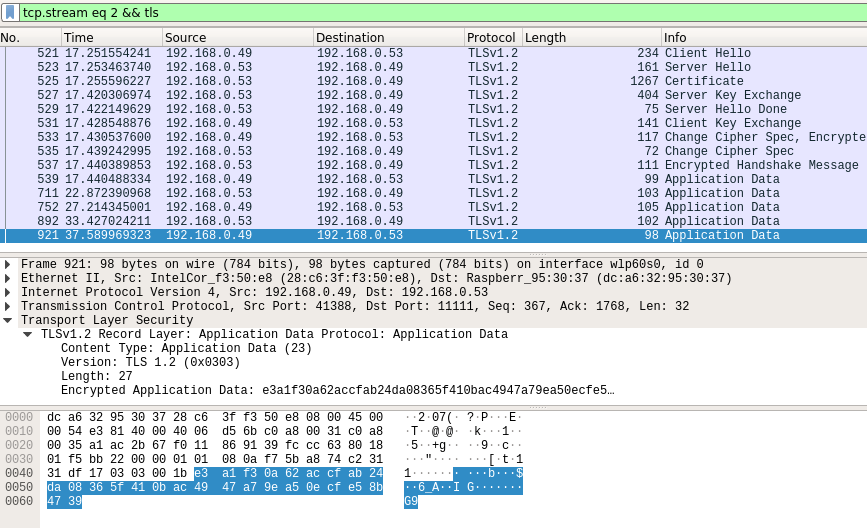
\includegraphics[scale=0.5]{./code/img/wireshark-iterative.png}
    \caption{Wireshark's screenshot}
    
\end{figure}
\subsubsection{Threaded program}
The threaded program is a TLS and TCP chat for 10 clients at most. It's a client-server program where multiple clients get connected to the server with a TLS socket and a TCP socket; the two sockets per client are used to show the difference, in the same program, between a communication with encryption and a communication without it.

This program is a chat where clients can send messages to other clients; they can choose between a single private message and a public message visible to all clients. 

To send a public message a client must only write a message with the keyboard and click enter. This message is sent with a TCP socket to the server; when the server receives a public message through a TCP socket, it sends the message to all TCP sockets connected with it, creating a broadcast communication.

When a client wants to send a private message to a connected client, before the message it must put the '\#' symbol, followed by the id of the client. To see all the clients id, a client must send 'list' command. The private message is sent with a TLS socket.
\subsubsection{Server threaded }
The server's main function after the setup of the TLS and TCP socket, it creates a thread to accept the incoming connections from clients.
\begin{lstlisting}[caption={int main() of TLS server},captionpos=b][language=c]
int main()
{
    /* Initialize wolfSSL */
    wolfSSL_Init();

    /* Create a socket that uses an internet IPv4 address,
     * Sets the socket to be stream based (TCP),
     * 0 means choose the default protocol. */
    if ((sockfd = socket(AF_INET, SOCK_STREAM, 0)) == -1)
    {
        fprintf(stderr, "ERROR: failed to create the socket\n");
        return -1;
    }
    if ((sockfdTCP = socket(AF_INET, SOCK_STREAM, 0)) == -1)
    {
        fprintf(stderr, "ERROR: failed to create the socket\n");
        return -1;
    }
    if (setsockopt(sockfd, SOL_SOCKET, SO_REUSEADDR, &(int){1}, sizeof(int)) < 0)
        printf("setsockopt(SO_REUSEADDR) failed");
    if (setsockopt(sockfdTCP, SOL_SOCKET, SO_REUSEADDR, &(int){1}, sizeof(int)) < 0)
        printf("setsockopt(SO_REUSEADDR) failed");
    /* Create and initialize WOLFSSL_CTX */

    if ((ctx = wolfSSL_CTX_new(wolfTLSv1_2_server_method())) == NULL)
    {
        fprintf(stderr, "ERROR: failed to create WOLFSSL_CTX\n");
        return -1;
    }

    /* Load server certificates into WOLFSSL_CTX */
    if (wolfSSL_CTX_use_certificate_file(ctx, CERT_FILE, SSL_FILETYPE_PEM) != SSL_SUCCESS)
    {
        fprintf(stderr, "ERROR: failed to load %s, please check the file.\n",
                CERT_FILE);
        return -1;
    }

    /* Load server key into WOLFSSL_CTX */
    if (wolfSSL_CTX_use_PrivateKey_file(ctx, KEY_FILE, SSL_FILETYPE_PEM) != SSL_SUCCESS)
    {
        fprintf(stderr, "ERROR: failed to load %s, please check the file.\n",
                KEY_FILE);
        return -1;
    }

    /* Initialize the server address struct with zeros */
    memset(&servAddr, 0, sizeof(servAddr));

    /* Fill in the server address */
    servAddr.sin_family = AF_INET;           /* using IPv4      */
    servAddr.sin_port = htons(DEFAULT_PORT); /* on DEFAULT_PORT */
    servAddr.sin_addr.s_addr = INADDR_ANY;   /* from anywhere   */

    /* Initialize the server address struct with zeros */
    memset(&servAddrTCP, 0, sizeof(servAddrTCP));

    /* Fill in the server address */
    servAddrTCP.sin_family = AF_INET;               /* using IPv4      */
    servAddrTCP.sin_port = htons(DEFAULT_PORT_TCP); /* on DEFAULT_PORT */
    servAddrTCP.sin_addr.s_addr = INADDR_ANY;       /* from anywhere   */

    /* Bind the server socket to our port */
    if (bind(sockfd, (struct sockaddr *)&servAddr, sizeof(servAddr)) == -1)
    {
        fprintf(stderr, "ERROR: failed to bind\n");
        return -1;
    }

    /* Bind the server socket to our port */
    if (bind(sockfdTCP, (struct sockaddr *)&servAddrTCP, sizeof(servAddrTCP)) == -1)
    {
        fprintf(stderr, "ERROR: failed to bind\n");
        return -1;
    }

    /* Listen for a new connection */
    if (listen(sockfd, 10) == -1)
    {
        fprintf(stderr, "ERROR: failed to listen\n");
        return -1;
    }

    /* Listen for a new connection */
    if (listen(sockfdTCP, 10) == -1)
    {
        fprintf(stderr, "ERROR: failed to listen\n");
        return -1;
    }

    if (pthread_create(&Taccept, NULL, acceptConnection, NULL))
    {
        fprintf(stderr, "Error creating thread\n");
        fflush(stdout);
        return -1;
    }

    pthread_join(Taccept, NULL);
    ncurses_end();
    return 0;
}
\end{lstlisting}
The \textbf{void *acceptConnection(void *args)} function is executed by a thread; the aim of this function is to accept incoming connections from TLS and TCP socket. When a TLS and a TCP connection are set, the server assigns an id to the client. After that, two threads are created to read from a TCP socket and a TLS socket.
\begin{lstlisting}[caption={void *acceptConnection(void *args) of TLS server},captionpos=b][language=c]
void *acceptConnection(void *args)
{
    int ret;
    ncurses_start();
    clearWin();
    while (1)
    {
        /* Accept client connections */
        clients[counter].size = sizeof(clients[counter].clientAddr);
        if ((clients[counter].connd = accept(sockfd, (struct sockaddr *)&clients[counter].clientAddr, &clients[counter].size)) == -1)
        {
            fprintf(stderr, "ERROR: failed to accept the connection\n\n");
            return NULL;
        }
        if ((clients[counter].conndTCP = accept(sockfdTCP, (struct sockaddr *)&clients[counter].clientAddr, &clients[counter].size)) == -1)
        {
            fprintf(stderr, "ERROR: failed to accept the connection\n\n");
            return NULL;
        }

        /* Create a WOLFSSL object */
        if ((clients[counter].ssl = wolfSSL_new(ctx)) == NULL)
        {
            fprintf(stderr, "ERROR: failed to create WOLFSSL object\n");
            return NULL;
        }

        /* Attach wolfSSL to the socket */
        wolfSSL_set_fd(clients[counter].ssl, clients[counter].connd);

        /* Establish TLS connection */
        ret = wolfSSL_accept(clients[counter].ssl);
        if (ret != SSL_SUCCESS)
        {
            ncurses_end();
            fprintf(stderr, "wolfSSL_accept error = %d\n",
                    wolfSSL_get_error(clients[counter].ssl, ret));
            return NULL;
        }
        printText("Client connected successfully\n", "System");
        int *argCounter = malloc(sizeof(*argCounter));
        if (argCounter == NULL)
        {
            fprintf(stderr, "Couldn't allocate memory for thread arg.\n");
            exit(EXIT_FAILURE);
        }

        *argCounter = counter;
        if (pthread_create(&Treader[counter], NULL, readBuffer, argCounter))
        {
            fprintf(stderr, "Error creating thread\n");
            fflush(stdout);
            return NULL;
        }
        if (pthread_create(&TreaderTCP[counter], NULL, readBufferTCP, argCounter))
        {
            fprintf(stderr, "Error creating thread\n");
            fflush(stdout);
            return NULL;
        }
        counter++;
    }
}
\end{lstlisting}
The \textbf{void *readBufferTCP(void *args)} function allows to read data from a TCP socket. In the program, there will be as many threads that execute this function as the number of connected clients; it reads messages from socket and it sends their content to all clients. This function will be executed until a client sends a 'quit' message or errors in socket occurred.
\begin{lstlisting}[caption={void *readBufferTCP(void *args) of TLS server},captionpos=b][language=c]
void *readBufferTCP(void *args)
{
    int ret;
    int id = *((int *)args);
    char output[256] = "";
    while (1)
    {
        memset(clients[id].buffReaderTCP, 0, sizeof(clients[id].buffReaderTCP));
        if (read(clients[id].conndTCP, clients[id].buffReaderTCP, sizeof(clients[id].buffReaderTCP)) <= 0)
        {
            fprintf(stderr, "ERROR: failed to read\n");
            pthread_cancel(TreaderTCP[id]);
            return NULL;
        }
        printText(clients[id].buffReaderTCP, clients[id].username);
        if (!strcmp(clients[id].buffReaderTCP, "quit"))
        {
            stopApplication();
            free(args);
            pthread_exit(NULL); /* End threaded execution                */
        }
        memset(output, 0, sizeof(output));
        for (int i = 0; i < counter; i++)
        {
            if (i != id)
            {
                strcat(output, clients[id].username);
                strcat(output, "`");
                strcat(output, clients[id].buffReaderTCP);
                ret = write(clients[i].conndTCP, output, XSTRLEN(output));
                if (ret <= 0)
                {
                    fprintf(stderr, "ERROR: failed to write\n");
                    pthread_cancel(TreaderTCP[id]);
                    return NULL;
                }
            }
        }
    }
}
\end{lstlisting}
The \textbf{void *readBuffer(void *args)} function is similar to the previous function; it reads data from a TLS socket, and it is used for receiving encrypted messages that they will be sent to a single client; this allows to create a single private chat between two clients.
\begin{lstlisting}[caption={void *readBuffer(void *args) of TLS server},captionpos=b][language=c]
void *readBuffer(void *args)
{
    int ret;
    int id = *((int *)args);
    //Read the username
    XMEMSET(clients[id].buffReader, 0, sizeof(clients[id].buffReader));
    ret = wolfSSL_read(clients[id].ssl, clients[id].buffReader, sizeof(clients[id].buffReader) - 1);
    strcpy(clients[id].username, clients[id].buffReader);

    while (1)
    {
        /* Read the client data into our buff array */
        XMEMSET(clients[id].buffReader, 0, sizeof(clients[id].buffReader));
        if (clients[id].ssl != NULL)
        {
            ret = wolfSSL_read(clients[id].ssl, clients[id].buffReader, sizeof(clients[id].buffReader) - 1);

            if (ret > 0)
            {
                if (!strcmp(clients[id].buffReader, "list"))
                {
                    wolfSSL_write(clients[id].ssl, "Server", XSTRLEN("Server"));
                    wolfSSL_write(clients[id].ssl, "Connected clients:", XSTRLEN("Connected clients:"));
                    for (int j = 0; j < counter; j++)
                    {
                        if (j != id)
                        {
                            char num[50];
                            sprintf(num, "%d", j);
                            wolfSSL_write(clients[id].ssl, num, XSTRLEN(num));
                            wolfSSL_write(clients[id].ssl, clients[j].username, XSTRLEN(clients[j].username));
                        }
                    }
                }
                else if (clients[id].buffReader[0] == '#')
                {
                    int dest = clients[id].buffReader[1] - 48; //ASCII
                    if (dest <= counter && dest >= 0)
                    {
                        char str[255];
                        strcpy(str, "private-");
                        strcat(str, clients[id].username);
                        ret = wolfSSL_write(clients[dest].ssl, str, XSTRLEN(str));
                        strcpy(str, clients[id].buffReader + 2);
                        ret = wolfSSL_write(clients[dest].ssl, str, XSTRLEN(str));
                    }
                }
            }
            else
            {
                printText("ERROR READ!!", "System");
                pthread_exit(NULL); /* End threaded execution                */
            }
        }
    }
    free(args);
}
\end{lstlisting}
\subsubsection{Client threaded}
The client's main function gets the server's IP address and then it creates a thread to setup the communication.
\begin{lstlisting}[caption={int main(int argc, char **argv) of TLS client},captionpos=b][language=c]
int main(int argc, char **argv)
{
    pthread_t Tclient;
    /* Check for proper calling convention */
    if (argc != 2)
    {
        printf("usage: %s <IPv4 address>\n", argv[0]);
        return -1;
    }

    ip = argv[1];

    /* create a second thread which executes inc_x(&x) */
    if (pthread_create(&Tclient, NULL, client, NULL))
    {

        fprintf(stderr, "Error creating thread\n");
        fflush(stdout);
        return 1;
    }

    if (pthread_join(Tclient, NULL))
    {

        fprintf(stderr, "Error joining thread\n");
        return 2;
    }
    ncurses_end();
    return 0; /* Return reporting a success               */
}
\end{lstlisting}
The \textbf{void *client(void *args)} function requests to the user an username and then it tries to connect to two different socket; the first one will be used in the public communication, instead the second one will be used to the private communication over a TLS socket.

When the sockets setup is done, the function sends the username to the server over TLS socket. At the end, three other threads will be created to handle the sending and receiving data over TCP and TLS sockets.
\begin{lstlisting}[caption={void *client(void*args) of TLS client},captionpos=b][language=c]
void *client(void *args)
{
    struct sockaddr_in servAddr;
    struct sockaddr_in servAddrTCP;

    printf("Set your username: ");
    refresh();
    if (!scanf("%s", username))
    {
        fprintf(stderr, "ERROR: failed to get message for server\n");
        return NULL;
    }
    ncurses_start();
    /* Initialize wolfSSL */
    wolfSSL_Init();

    /* Create a socket that uses an internet IPv4 address,
     * Sets the socket to be stream based (TCP),
     * 0 means choose the default protocol. */
    if ((sockfd = socket(AF_INET, SOCK_STREAM, 0)) == -1)
    {
        fprintf(stderr, "ERROR: failed to create the socket\n");
        return NULL;
    }
    if ((sockfdTCP = socket(AF_INET, SOCK_STREAM, 0)) == -1)
    {
        fprintf(stderr, "ERROR: failed to create the socket\n");
        return NULL;
    }

    /* Create and initialize WOLFSSL_CTX */
    if ((ctx = wolfSSL_CTX_new(wolfTLSv1_2_client_method())) == NULL)
    {
        fprintf(stderr, "ERROR: failed to create WOLFSSL_CTX\n");
        return NULL;
    }

    /* Load client certificates into WOLFSSL_CTX */
    if (wolfSSL_CTX_load_verify_locations(ctx, CERT_FILE, NULL) != SSL_SUCCESS)
    {
        fprintf(stderr, "ERROR: failed to load %s, please check the file.\n",
                CERT_FILE);
        return NULL;
    }

    /* Initialize the server address struct with zeros */
    memset(&servAddr, 0, sizeof(servAddr));

    /* Fill in the server address */
    servAddr.sin_family = AF_INET;           /* using IPv4      */
    servAddr.sin_port = htons(DEFAULT_PORT); /* on DEFAULT_PORT */

    /* Initialize the server address struct with zeros */
    memset(&servAddrTCP, 0, sizeof(servAddrTCP));

    /* Fill in the server address */
    servAddrTCP.sin_family = AF_INET;               /* using IPv4      */
    servAddrTCP.sin_port = htons(DEFAULT_PORT_TCP); /* on DEFAULT_PORT */

    /* Get the server IPv4 address from the command line call */
    if (inet_pton(AF_INET, ip, &servAddr.sin_addr) != 1)
    {
        fprintf(stderr, "ERROR: invalid address\n");
        return NULL;
    }

    /* Get the server IPv4 address from the command line call */
    if (inet_pton(AF_INET, ip, &servAddrTCP.sin_addr) != 1)
    {
        fprintf(stderr, "ERROR: invalid address\n");
        return NULL;
    }

    /* Connect to the server */

    if (connect(sockfd, (struct sockaddr *)&servAddr, sizeof(servAddr)) == -1)
    {
        printText("ERROR: failed to connect", "System");
        return NULL;
    }

    /* Connect to the server */

    if (connect(sockfdTCP, (struct sockaddr *)&servAddrTCP, sizeof(servAddrTCP)) == -1)
    {
        printText("ERROR: failed to connect", "System");
        return NULL;
    }

    /* Create a WOLFSSL object */
    if ((ssl = wolfSSL_new(ctx)) == NULL)
    {
        fprintf(stderr, "ERROR: failed to create WOLFSSL object\n");
        return NULL;
    }

    /* Attach wolfSSL to the socket */
    wolfSSL_set_fd(ssl, sockfd);
    /* Connect to wolfSSL on the server side */
    if (wolfSSL_connect(ssl) != SSL_SUCCESS)
    {
        fprintf(stderr, "ERROR: failed to connect to wolfSSL\n");
        return NULL;
    }

    strtok(username, "\n");
    len = strnlen(username, sizeof(username));
    /* Send the username to the server */
    if (wolfSSL_write(ssl, username, len) != len)
    {
        fprintf(stderr, "ERROR: failed to write\n");
        return NULL;
    }

    if (pthread_create(&Twriter, NULL, writeBuffer, NULL))
    {
        fprintf(stderr, "Error creating thread\n");
        fflush(stdout);
        return NULL;
    }

    if (pthread_create(&Treader, NULL, readBuffer, NULL))
    {
        fprintf(stderr, "Error creating thread\n");
        fflush(stdout);
        return NULL;
    }

    if (pthread_create(&TreaderTCP, NULL, readBufferTCP, NULL))
    {
        fprintf(stderr, "Error creating thread\n");
        fflush(stdout);
        return NULL;
    }

    pthread_join(Twriter, NULL);
    pthread_join(Treader, NULL);
    pthread_join(TreaderTCP,NULL);

    /* Cleanup and return */
    wolfSSL_free(ssl);     /* Free the wolfSSL object                  */
    wolfSSL_CTX_free(ctx); /* Free the wolfSSL context object          */
    wolfSSL_Cleanup();     /* Cleanup the wolfSSL environment          */
    close(sockfd);         /* Close the connection to the server       */
    printText("Communication is ended!\n Press a button!!!", "System");
    getch();
    return NULL;
}
\end{lstlisting}
The \textbf{void *writeBuffer(void *args)} function is used to write data in the right socket; it reads data written by the client with read\_in() function; if the message written by the client is "list" or the first character is "\#", the message will be sent over the TLS socket, otherwise the message will be sent over the TCP socket.
\begin{lstlisting}[caption={void *writeBuffer(void *args) of TLS client},captionpos=b][language=c]
void *writeBuffer(void *args)
{
    while (!is_end)
    {
        /* Get a message for the server from stdin */
        memset(Rbuffer, 0, sizeof(Rbuffer));
        read_in();
        len = strnlen(Rbuffer, sizeof(Rbuffer));
        if (XSTRNCMP(Rbuffer, "quit", 4) == 0)
        {
            if (write(sockfdTCP, Rbuffer, len) != len)
            {
                fprintf(stderr, "ERROR: failed to write\n");
                return NULL;
            }
            is_end = 1;
            pthread_cancel(Treader);
            pthread_cancel(TreaderTCP);
        }
        else if (XSTRNCMP(Rbuffer, "list", 4) == 0 || Rbuffer[0] == '#')
        {
            //wolfSSL_read
            /* Send the message to the server */
            if (wolfSSL_write(ssl, Rbuffer, len) != len)
            {
                fprintf(stderr, "ERROR: failed to write\n");
                return NULL;
            }
        }
        else
        {
            if (write(sockfdTCP, Rbuffer, len) != len)
            {
                fprintf(stderr, "ERROR: failed to write\n");
                return NULL;
            }
        }

        printText(Rbuffer, username);
    }
    return NULL;
}
\end{lstlisting}
The \textbf{void *readBuffer(void *args)} function reads the username and the message of the sender in the TLS socket, and it prints them in the GUI.
\begin{lstlisting}[caption={void *readBuffer(void *args) of TLS client},captionpos=b][language=c]
void *readBuffer(void *args)
{
    char username[256];
    while (!is_end)
    {
        /* Read the server data into our buff array */
        memset(buffReader, 0, sizeof(buffReader));
        if (wolfSSL_read(ssl, buffReader, sizeof(buffReader) - 1) == -1)
        {
            pthread_cancel(Twriter);
            return NULL;
        }
        strcpy(username, buffReader);
        memset(buffReader, 0, sizeof(buffReader));
        if (wolfSSL_read(ssl, buffReader, sizeof(buffReader) - 1) == -1)
        {
            pthread_cancel(Twriter);
            return NULL;
        }
        else
        {
            printText(buffReader, username);
        }
    }
    return NULL;
}
\end{lstlisting}
The \textbf{void *readBufferTCP(void *args)} do the same things of the previous function but it uses a TCP socket.
\begin{lstlisting}[caption={void *readBufferTCP(void *args) of TLS client},captionpos=b][language=c]
void *readBufferTCP(void *args)
{
    char username[50] = "";
    char output[256] = "";
    int ret;
    while (!is_end)
    {
        memset(buffReaderTCP, 0, sizeof(buffReaderTCP));
        memset(username, 0, sizeof(username));
        memset(output, 0, sizeof(output));
        ret = read(sockfdTCP, buffReaderTCP, sizeof(buffReaderTCP) - 1);
        if (ret <= 0)
        {
            pthread_cancel(TreaderTCP);
            return NULL;
        }
        getSenderUsername(buffReaderTCP, username);
        strcpy(output, getSenderData(buffReaderTCP,output));
        printText(output, username);
    }
    return NULL;
}
\end{lstlisting}

\subsection{Compile a WolfSSL program}
To execute a wolfSSL program you must have installed wolfSSL on your pc, and then you must add \textbf{-lwolfssl} on your gcc command.

In this program I used threads and ncurses so I had to add \textbf{-pthread} and \textbf{-lncurses} flags to gcc command; to optimize the compilation I created a makefile.

\subsection{Execute a WolfSSL program (threaded program)}
In my project I used a laptop for the client part, and a Raspberry Pi for the server part; they are connected to the same LAN.
In the pictures below you can see the GUI of the client and the server part, and the traffic analyze with wireshark.
The IP address of the server is \textbf{192.168.0.53}; the port for the TLS socket is \textbf{11111} and the port for the TCP socket is \textbf{11112}.
The IP address of the clients is \textbf{192.168.0.46} because I only had a PC and a raspberry to test the program.

\begin{figure}[H]
\begin{Verbatim}[commandchars=\\\{\}]
\textcolor{green}{pi@raspberrypi}\textcolor{black}{:}\textcolor{blue}{~/project-wolfssl/code/wolfSSL $}\textcolor{black}{./server-tls-threaded}
\textcolor{black}{Waiting for a connection...}
\end{Verbatim}
\caption{Execute WolfSSL server}
\end{figure}


\begin{figure}[H]
\begin{Verbatim}[commandchars=\\\{\}]
\textcolor{green}{luca@luca}\textcolor{black}{:}\textcolor{blue}{~/project-wolfssl/code/wolfSSL$}\textcolor{black}{./client-tls
-threaded}
\textcolor{black}{192.168.0.53}
\textcolor{black}{Set your username: }
\end{Verbatim}
\caption{Execute WolfSSL client}
\end{figure}

After the execution of the server, a client can connect to it and the ssl handshake starts.

With the hello packet below, the client provides an ordered list of 24 cipher suites that it will support for encryption. The list is in the order preferred by the client, with highest preference first. This list can be modified by the programmer.

In this case, the client provides a list of optional extension which the server can use to take action or enable new features, for example:
\begin{itemize}
\item signature\_algorithms
\begin{itemize}
\item The purpose of this extension is to allow clients to indicate to the server which signature/hash algorithm pairs may be used in digital signatures.
\end{itemize}
\end{itemize}
\begin{figure}[H]
    \centering
    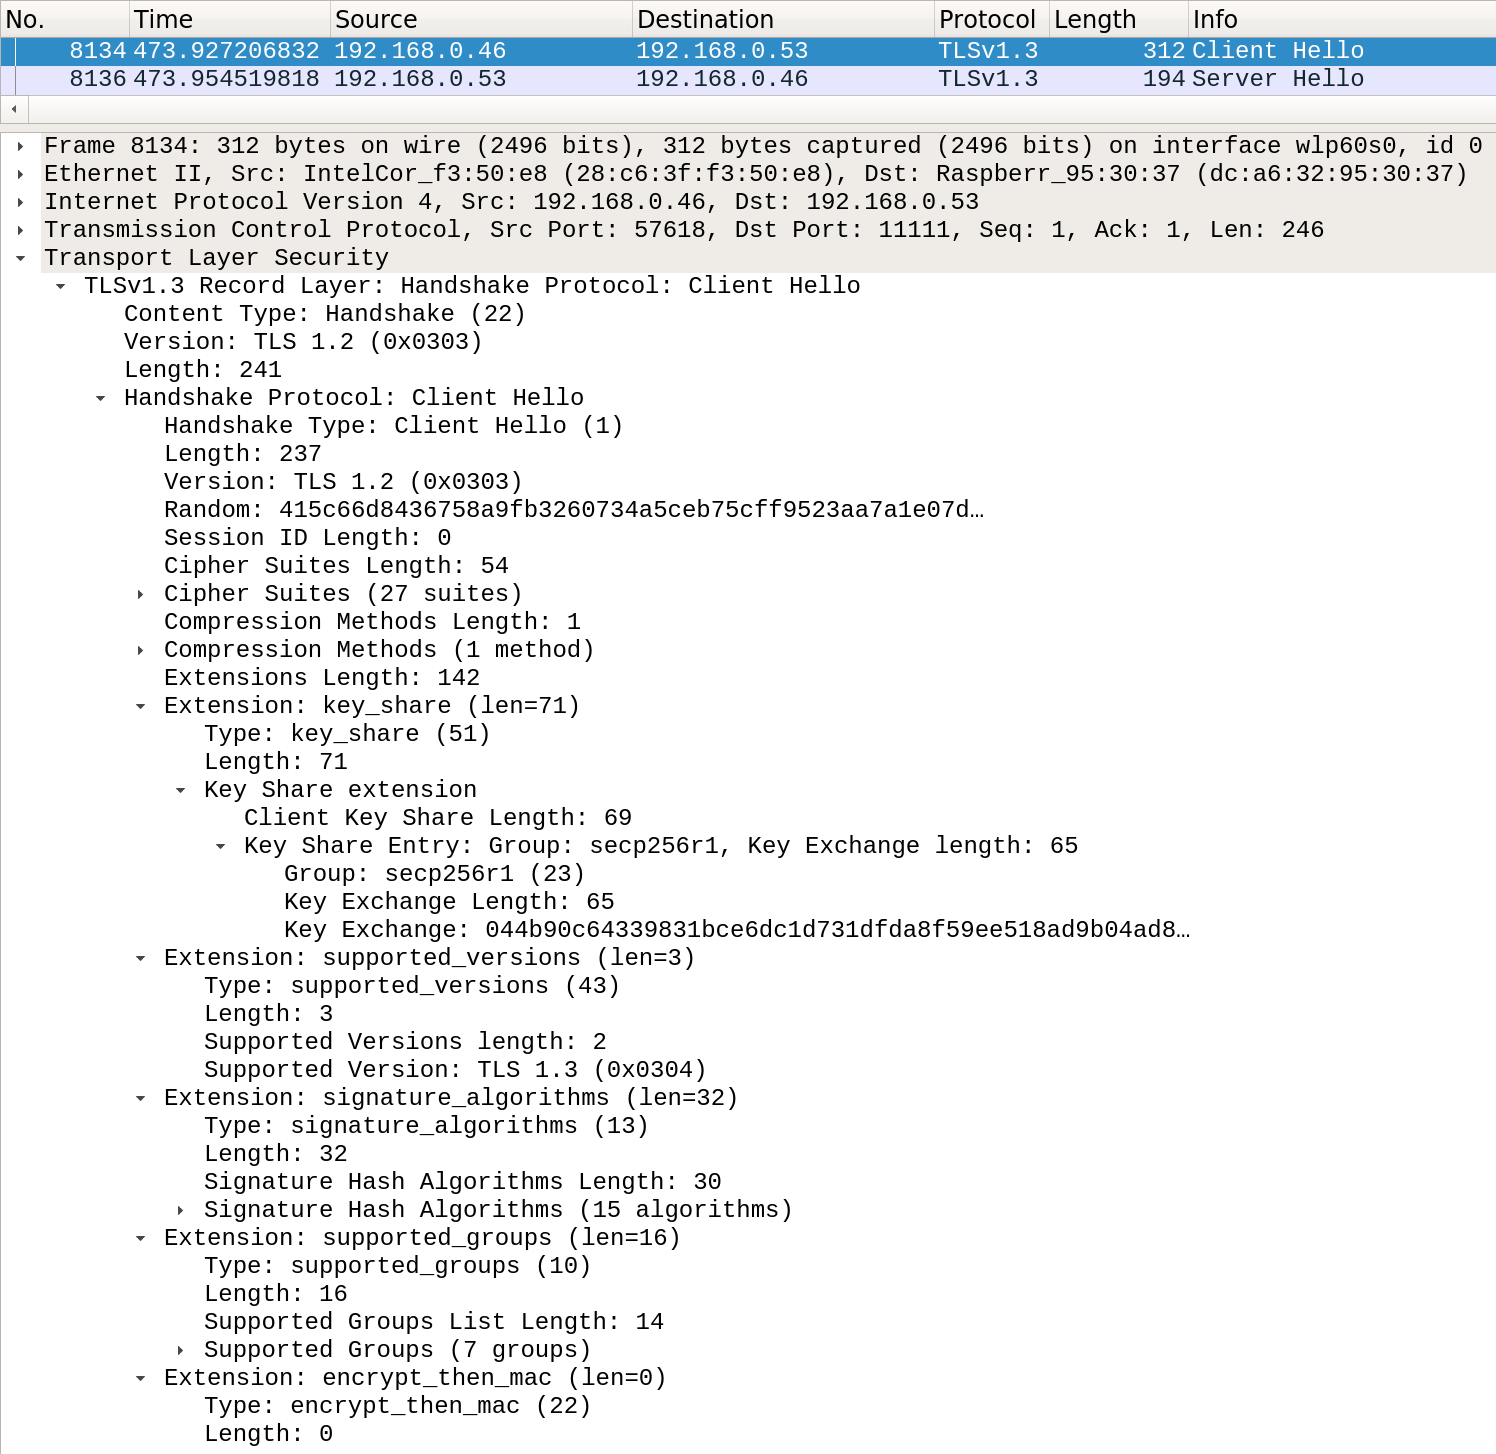
\includegraphics[scale=0.500]{./code/img/client-hello.png}
    \caption{Client Hello}
\end{figure}


In the Server Hello packet, the server has selected cipher suite 0xc030 (TLS\_ECDHE\_RSA\_WITH\_AES\_256\_GCM\_SHA384) from the list of options given by the client.

Random is 32-byte random number used to generate the Master Secret.

The session identifier is a unique number to identify the session for the corresponding connection with the client.

\begin{figure}[H]
    \centering
    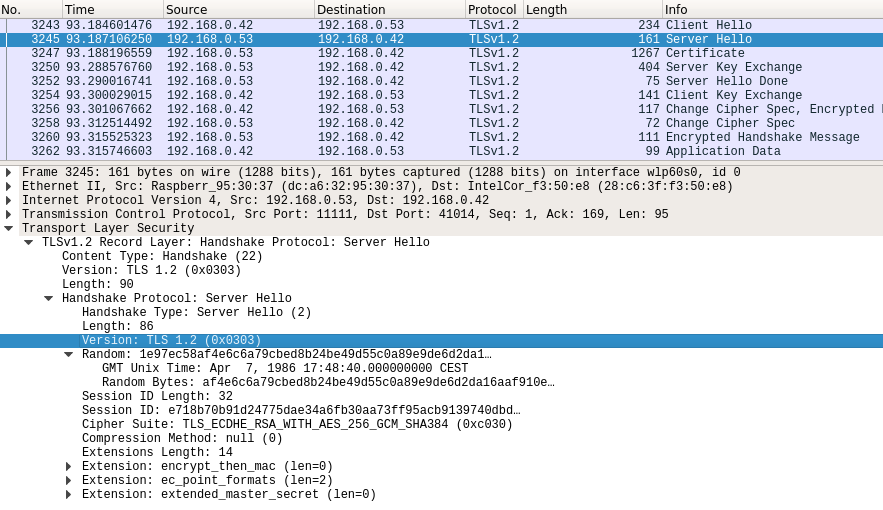
\includegraphics[scale=0.500]{./code/img/server-hello.png}
    \caption{Server Hello}
    
\end{figure}
The server sends the client a list of certificates to authenticate itself.
\begin{figure}[H]
    \centering
    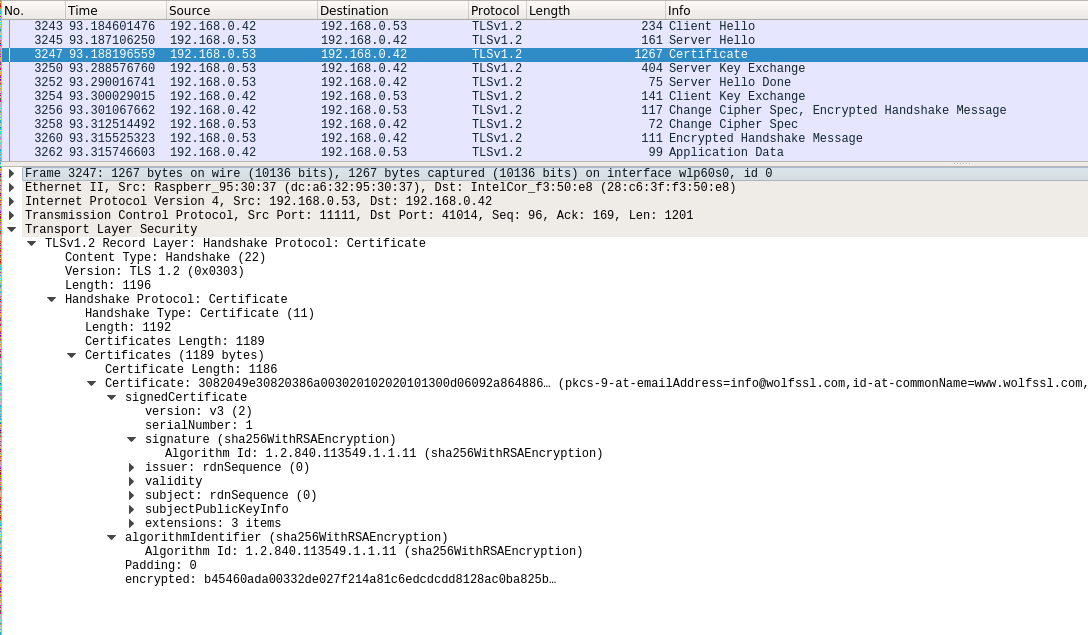
\includegraphics[scale=0.400]{./code/img/server-certificate.png}
    \caption{Server Certificate}
    
\end{figure}
The message \textbf{Server Key Exchange} is optional and sent when the public key present in the server's certificate is not suitable for key exchange, or if the cipher suite places a restriction requiring a temporary key. This key is used by the client to encrypt Client Key Exchange later in the process.
\begin{figure}[H]
    \centering
    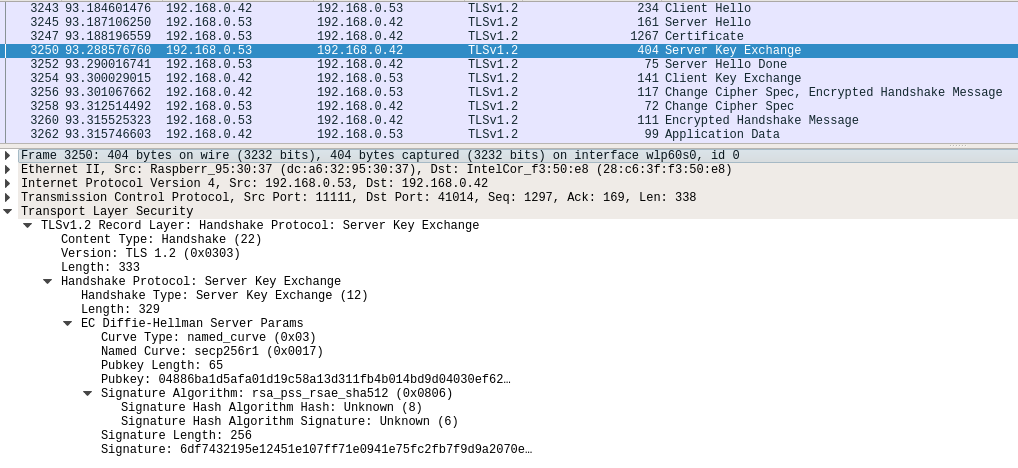
\includegraphics[scale=0.400]{./code/img/server-key-exchange.png}
    \caption{Server Key Exchange}
    
\end{figure}
This message indicates the server is done and is awaiting the client's response.
\begin{figure}[H]
    \centering
    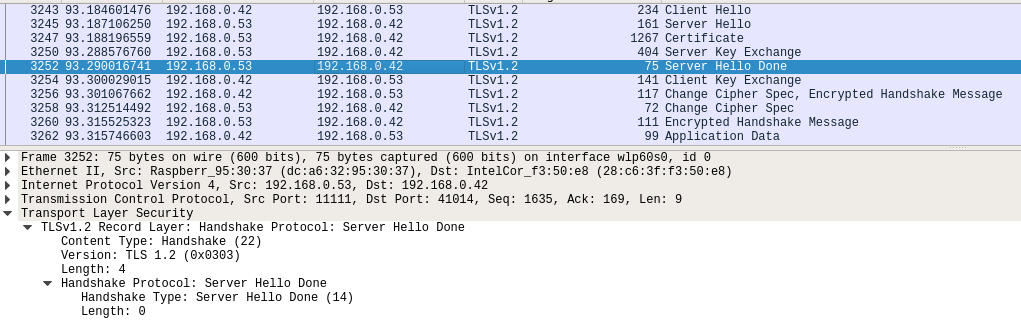
\includegraphics[scale=0.400]{./code/img/server-hello-done.png}
    \caption{Server Hello Done}
\end{figure}
The \textbf{Client Key Exchange} message contains the protocol version of the client which the server verifies if it matches with the original client hello message. It also has the pre-master secret; it is a random number generated by the client and encrypted with the server public key. This along with the client and server random number is used to create the master secret. If the server can decrypt the message using the private key and can create the master secret locally, then the client is assured that the server has authenticated itself.
\begin{figure}[H]
    \centering
    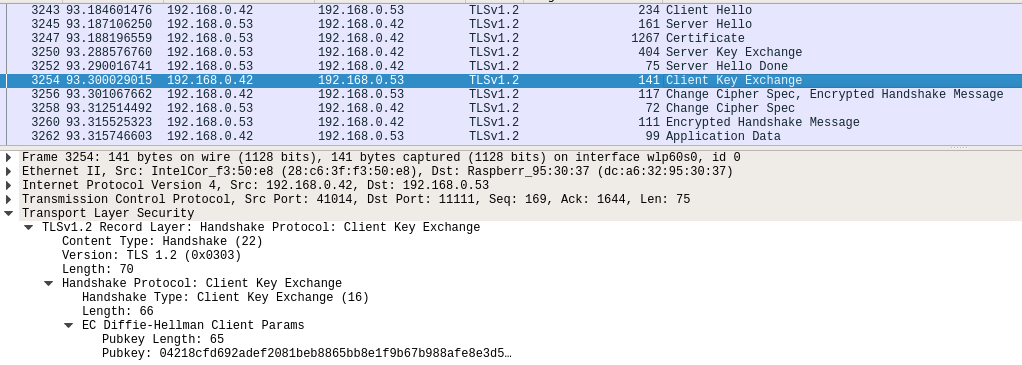
\includegraphics[scale=0.400]{./code/img/client-key-exchange.png}
    \caption{Client Key Exchange}
\end{figure}
The \textbf{Change Cipher Spec} message notifies the server that all the future messages will be encrypted using the algorithm and keys that were just negotiated.

The \textbf{Encrypted Handshake} message indicates that the TLS negotiations is completed for the client.
\begin{figure}[H]
    \centering
    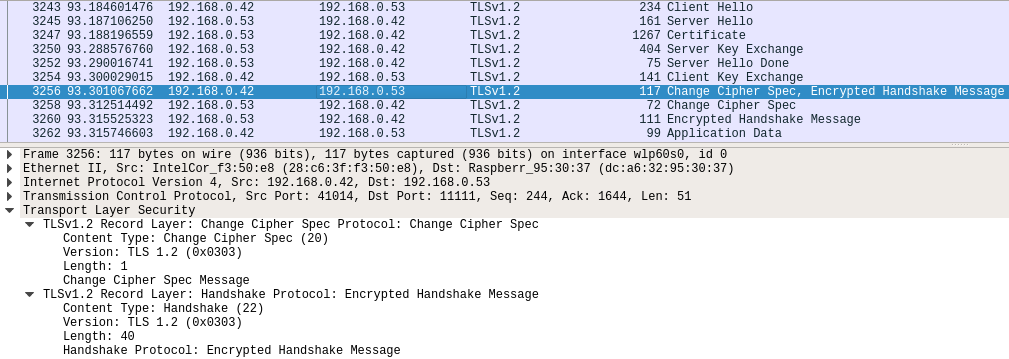
\includegraphics[scale=0.400]{./code/img/client-change-cipher.png}
    \caption{Change Cipher Spec and Encrypted Handshake}
\end{figure}

\textbf{(Change Cipher Spec)}The server informs the client that the messages will be encrypted with the existing algorithms and keys.
\begin{figure}[H]
    \centering
    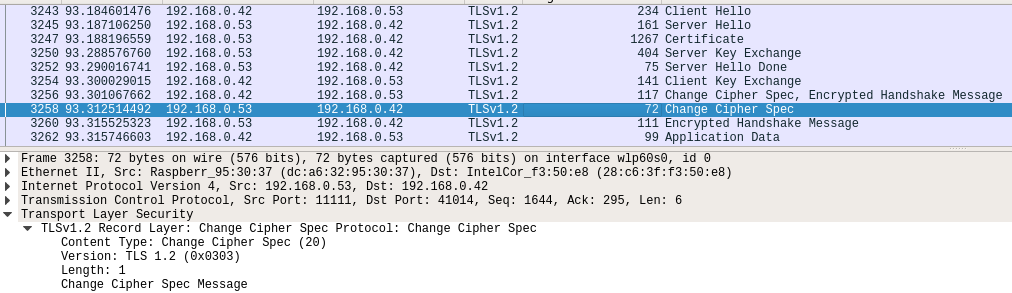
\includegraphics[scale=0.400]{./code/img/server-change-cipher.png}
    \caption{Change Cipher Spec}
\end{figure}
\textbf{(Encrypted Handshake Message)}Server informs the client the end of the TLS negotiations. It is like the client finished message.
\begin{figure}[H]
    \centering
    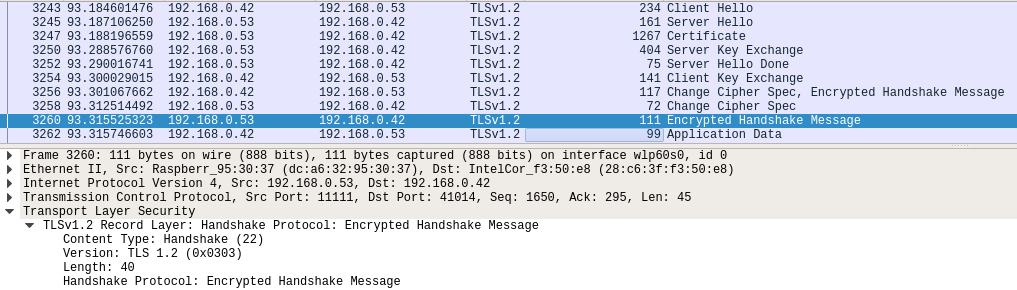
\includegraphics[scale=0.400]{./code/img/encrypted-handshake.png}
    \caption{Encrypted Handshake}
\end{figure}
Every client will do the same handshake described above.
After all clients' SSL handshake the situation in the server GUI is:
\begin{figure}[H]
\begin{Verbatim}[commandchars=\\\{\}]

|--------------------------\textcolor{orange}{WolfSSL chat}------------------------|
[System] Client Luca connected successfully                           
[System] ***************************                                        
[System] Client Maria connected successfully                           
[System] ***************************                                          
[System] Client Carlos connected successfully                           
[System] ***************************                                                                      
______________________________________________________________|
\end{Verbatim}
\caption{Connected clients, server GUI}
\end{figure}



To test the exact functioning of the program, I sent several messages.
\begin{figure}[H]
\begin{Verbatim}[commandchars=\\\{\}]

|--------------------------\textcolor{orange}{WolfSSL chat}------------------------|
[Luca] Hi                          
[Maria] Hi Luca!
[Carlos] Hi everyone!
[Luca] This message is public
[Luca] list
[Server] Connected clients:
[1] Maria
[2] Carlos
[Luca] #1 this message is only for you, Maria!
[private-Maria] Thank you Luca
______________________________________________________________|
\end{Verbatim}
\caption{Client Luca, GUI}
\end{figure}

\begin{figure}[H]
\begin{Verbatim}[commandchars=\\\{\}]
|--------------------------\textcolor{orange}{WolfSSL chat}------------------------|
[Luca] Hi                          
[Maria] Hi Luca!
[Carlos] Hi everyone!
[Luca] This message is public
[private-Luca] this message is only for you, Maria!
[Maria] list
[Server] Connected clients:
[0] Luca
[2] Carlos
[Maria] #0 Thank you Luca
[private-Maria] Thank you Luca
______________________________________________________________|
\end{Verbatim}
\caption{Client Maria, GUI}
\end{figure}

\begin{figure}[H]
\begin{Verbatim}[commandchars=\\\{\}]
|--------------------------\textcolor{orange}{WolfSSL chat}------------------------|
[Luca] Hi                          
[Maria] Hi Luca!
[Carlos] Hi everyone!
[Luca] This message is public
______________________________________________________________|
\end{Verbatim}
\caption{Client Carlos, GUI}
\end{figure}

With Wireshark you can see the difference between the TCP and TLS packets:
\begin{figure}[H]
    \centering
    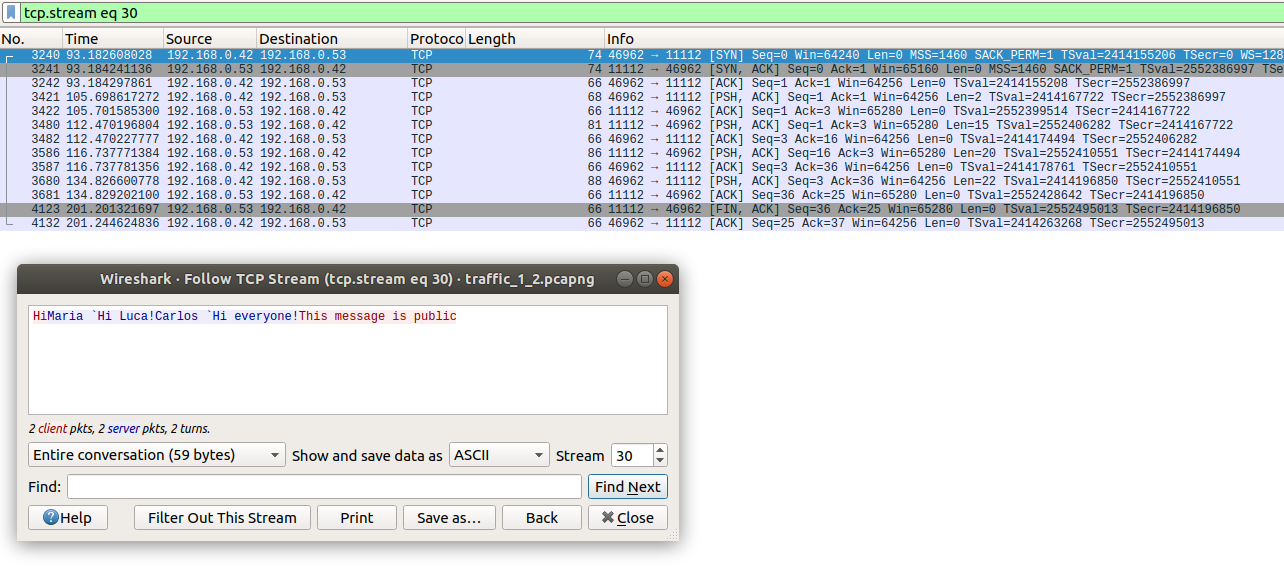
\includegraphics[scale=0.3]{./code/img/tcp-traffic.png}
    \caption{TCP traffic}
\end{figure}
In the TLS capture, after the handshake for each client, the messages are encrypted.
\begin{figure}[H]
    \centering
    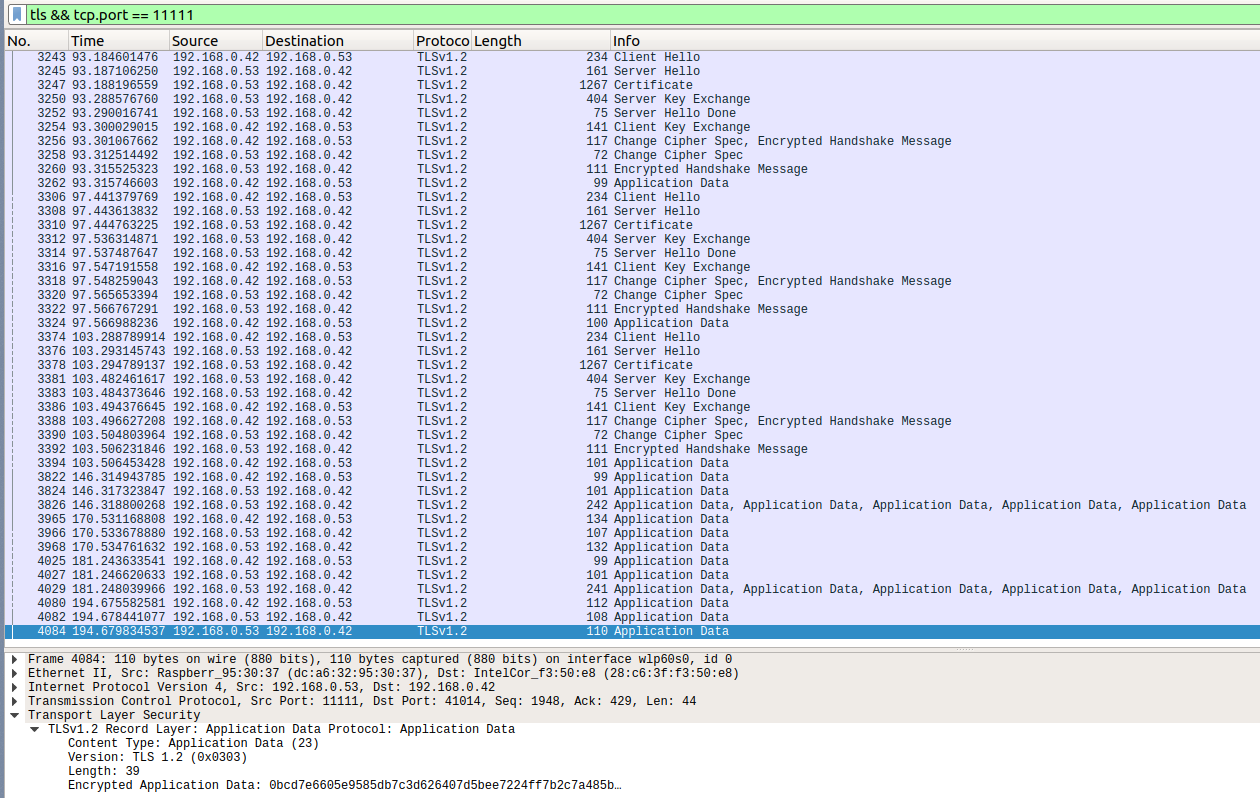
\includegraphics[scale=0.3]{./code/img/tls-traffic.png}
    \caption{TLS traffic}
\end{figure}


\section{Differences between WolfSSL and OpenSSL}
\subsection{Differences}

The main differences are:
\begin{itemize}
\item Memory Usage
\begin{itemize}
\item WolfSSL can be up to 20 times smaller than OpenSSL; The build size is between 20 and 100 KB and the runtime memory usage between 1 and 36 KB. This gives a major advantage of integrating in smaller embedded devices. 
\end{itemize}
\item Hardware Crypto
\begin{itemize}
\item WolfSSL has a partnership with the most MCU manufacturers which allows to be quite early in the market to support hardware acceleration on huge list of platforms.
\end{itemize}
\item Portability
\begin{itemize}
\item WolfSSL is more portable than OpenSSL because is made for real-time, mobile, embedded and enterprise systems.
\end{itemize}
\end{itemize}

\subsection{Build size and speed test}
I downloaded openSSL (version: 3.0.0-alpha7-dev) and wolfSSL (version: 4.5.0) in a Raspberry Pi 4 and I noticed the difference in terms of space occupied.
OpenSSL occupies 412.5 MB while wolfSSL only 47 MB. This difference also affects the compilation and installation time; WolfSSL is compiled and installed in about 3 minutes while openSSL takes at least 10 minutes.
The wolfSSL and openSSL libraries are installed in /usr/local/lib directory and occupied respectively 0.37 MB and 11 MB.
WolfSSL provides 263 possibilities circa of custom installation; these flags allow the user to choose the enabling or disabling wolfSSL features. Different features can reduce or increase the space occupancy on the disk, for example, enabling all wolfSSL features the library is 1.2 MB.
To reduce the size of wolfSSL library I tried to configure it by disabling some cipher algorithms and other wolfSSL features with these flags:

\textit{--disable-aes --disable-aescbc --disable-aesgcm --disable-asm --enable-chacha --disable-crypttests --disable-des3 --enable-dh --disable-ecc --disable-eccshamir --disable-errorstrings --disable-examples --disable-inline --disable-md5 --disable-memory --disable-oldnames --disable-oldtls --enable-poly1305 --disable-sha224 --disable-sha512 --disable-base64encode --disable-extended-master --disable-harden --disable-jobserver}

This configuration produces a wolfSSL library that occupies 0.26 MB on disk.

Wolfssl is definitely made for embedded systems, but how much can the data forwarding performance differ?
\\To answer this question I created two program that exchange data between a Raspberry and a laptop, one for wolfSSL and one for openSSL. In the specification, one of the two reads a file and sends the read content to the other one.
The two programs are identical, the only difference are the function calls. One program has the functions of openssl and the other of wolfssl.
\\For the wolfSSL I used the same certificates and key used in the previous program, while for the openSSL I created a root CA certificate, a server key and a certificate signing request with these commands:
\begin{lstlisting}[caption={openSSL commands},captionpos=b][language=bash]
openssl genrsa -des3 -out CA-key.pem 2048
openssl req -new -key CA-key.pem -x509 -days 1000 -out CA-cert.pem
openssl genrsa -des3 -out server-key.pem 2048
openssl req ?new ?config openssl.cnf ?key server-key.pem ?out signingReq.csr
openssl x509 -req -days 365 -in signingReq.csr -CA CA-cert.pem -CAkey CA-key.pem -CAcreateserial -out server-cert.pem
\end{lstlisting}

I created these programs to measure the data forwarding time.

The functions under examination are writefile (receive data from the secure channel) and sendfile (send data through the secure channel):

\begin{lstlisting}[caption={sendfile openSSL function},captionpos=b][language=c]
void sendfile(FILE *fp, SSL *ssl)
{
    int n;
    char sendline[MAX_LINE];
    clock_t t, sum = 0;
    t = clock();
    while ((n = fread(sendline, sizeof(char), MAX_LINE - 1, fp)) > 0)
    {
        if (n != MAX_LINE && ferror(fp))
        {
            perror("Read File Error");
            exit(1);
        }
        t = clock();
        if ((total += SSL_write(ssl, sendline, strlen(sendline))) < 0)
        {
            perror("Can't send file");
            exit(1);
        }
        sum += clock() - t;
        memset(sendline, 0, MAX_LINE);
    }
    double time_taken = ((double)sum) / CLOCKS_PER_SEC; // in seconds
    printf("%f seconds to send data \n", time_taken);
}
\end{lstlisting}

\begin{lstlisting}[caption={writefile openSSL function},captionpos=b][language=c]
void writefile(SSL *ssl, FILE *fp)
{
    ssize_t n;
    char buff[MAX_LINE] = {0};
    clock_t t,sum = 0;
    t = clock();
    while ((n = SSL_read(ssl, buff, sizeof(buff))) > 0)
    {
        sum += clock() - t;
        total += n;
        if (n == -1)
        {
            perror("Receive File Error");
            exit(1);
        }
        if (fwrite(buff, sizeof(char), n, fp) != n)
        {
            perror("Write File Error");
            exit(1);
        }
        memset(buff, 0, MAX_LINE);
        t = clock();
    }
    double time_taken = ((double)sum) / CLOCKS_PER_SEC; // in seconds
    printf("%f seconds to receive data \n", time_taken);
}

\end{lstlisting}

\begin{lstlisting}[caption={sendfile wolfSSL function},captionpos=b][language=c]
void sendfile(FILE *fp, WOLFSSL *ssl)
{
    int n;
    char sendline[MAX_LINE];
    clock_t t, sum = 0;
    t = clock();
    while ((n = fread(sendline, sizeof(char), MAX_LINE - 1, fp)) > 0)
    {
        if (n != MAX_LINE && ferror(fp))
        {
            perror("Read File Error");
            exit(1);
        }
        t = clock();
        if ((total += wolfSSL_write(ssl, sendline, strlen(sendline))) < 0)
        {
            perror("Can't send file");
            exit(1);
        }
        sum += clock() - t;
        memset(sendline, 0, MAX_LINE);
    }
    double time_taken = ((double)sum) / CLOCKS_PER_SEC; // in seconds
    printf("%f seconds to send data \n", time_taken);
}

\end{lstlisting}

\begin{lstlisting}[caption={writefile wolfSSL function},captionpos=b][language=c]
void writefile(WOLFSSL *ssl, FILE *fp)
{
    ssize_t n;
    char buff[MAX_LINE] = {0};
    clock_t t,sum = 0;
    t = clock();
    while ((n = wolfSSL_read(ssl, buff, sizeof(buff))) > 0)
    {
        sum += clock() - t;
        total += n;
        if (n == -1)
        {
            perror("Receive File Error");
            exit(1);
        }
        if (fwrite(buff, sizeof(char), n, fp) != n)
        {
            perror("Write File Error");
            exit(1);
        }
        memset(buff, 0, MAX_LINE);
        t = clock();
    }
    double time_taken = ((double)sum) / CLOCKS_PER_SEC; // in seconds
    printf("%f seconds to receive data \n", time_taken);
}
\end{lstlisting}
The rest of the code is on github.

For the following test I created 4 files size about 128 MB, 256 MB, 512 MB and 1 GB with these commands:
\begin{lstlisting}[caption={openSSL commands},captionpos=b][language=bash]
128 MB = ./random.sh 128000000
256 MB = ./random.sh 256000000
512 MB = ./random.sh 512000000
1 GB = ./random.sh 1000000000
\end{lstlisting}

This test is made in my gigabit home network.
The time is in seconds.
\\The cipher suite used is: TLS\_ECDHE\_RSA\_WITH\_AES\_256\_GCM\_SHA384

Send file:\\
\begin{tabular}{ ||c|c|c|c|c|| } 
 \hline
 \textbf{openSSL} & time1 & time2 & time3 & average \\ 
 \hline
 128 MB & 0.18& 0.25& 0.21& 0.21\\ 
 \hline
 256 MB & 0.56& 0.42& 0.45& 0.48\\ 
 \hline
 512 MB & 1.13& 1.06& 0.77& 0.99\\ 
 \hline
 1 GB  & 1.74& 1.69& 1.53& 1.65\\ 
 \hline
\end{tabular}
\newline
\begin{tabular}{ ||c|c|c|c|c|| } 
 \hline
 \textbf{wolfSSL} & time1 & time2 & time3 & average \\ 
 \hline
128 MB & 5.40& 5.36& 4.64& 5.13\\ 
 \hline
 256 MB & 10.59& 8.69& 8.89& 9.39\\ 
 \hline
 512 MB & 20.73& 20.88& 22.16& 21.26\\ 
 \hline
 1 GB  & 40.94& 36.84& 35.58& 37.79\\ 
 \hline
\end{tabular}
\newline

Receive file:\\
\begin{tabular}{ ||c|c|c|c|c|| } 
 \hline
 \textbf{openSSL} & time1 & time2 & time3 & average \\ 
 \hline
 128 MB & 3.61& 3.89& 3.59& 3.70\\ 
 \hline
 256 MB & 7.08& 7.30& 7.24& 7.21\\ 
 \hline
 512 MB & 15.73& 16.65& 14.56& 15.65\\ 
 \hline
 1 GB  & 29.86& 29.26& 28.42& 29.18\\ 
 \hline
\end{tabular}
\newline
\begin{tabular}{ ||c|c|c|c|c|| } 
 \hline
 \textbf{wolfSSL} & time1 & time2 & time3 & average \\ 
 \hline
128 MB & 12.53& 13.33& 13.83& 13.23\\ 
 \hline
 256 MB & 25.09& 25.02& 25.05& 25.05\\ 
 \hline
 512 MB & 51.15& 50.83& 53.30& 51.76\\ 
 \hline
 1 GB  & 97.85& 97.78& 98.62& 98.08\\ 
 \hline
\end{tabular}
\newline

OpenSSL is more performing than wolfssl; the difference of time is relevant.
Sending large amounts of data you can see the difference between them, but wolfSSL being born for embedded systems works very well and above all it takes up less space.

\subsection{Run-time memory occupation}
To compare the run-time memory occupation between openSSL and wolfSSL I used the linux task manager and valgrind. Using the task manager, the values aren't the exactly run-time memory occupation in a precise moment but the memory reserved by the operating system for the process; this allows me to do an estimation and a comparison among them.

In this comparison I monitored the RSS and the VSZ:
the RSS is the Resident Set Size and it is used to show how much memory is allocated to that process in RAM. It does not include memory that is swapped out. It includes memory from shared libraries as long as the pages from those libraries are actually in memory. It also includes all stack and heap memory.
The VSZ is the Virtual Memory Size. It includes all memory that the process can access, including memory that is swapped out, memory that is allocated, but not used, and memory that is from shared libraries.

The run-time memory occupation of the receive program (writefile function) is:
\\
\begin{tabular}{ ||c|c|c|c|c|| } 
 \hline
 & RSS & VSZ\\ 
 \hline
 \textbf{wolfSSL} &1.3 MB& 12.6MB\\ 
 \hline
 \textbf{openSSL} &5.9 MB& 18.2MB\\ 
 \hline
\end{tabular}
\newline
\newline
With valgrind the total heap usage by openSSL is: 23,947 allocs, 23,947 frees, 6,937,196 bytes allocated.
The total heap usage by wolfSSL is: 104 allocs, 104 frees, 121,036 bytes allocated.

Even in a small program the difference is relevant.

\subsection{Segment size comparison}
In order to compare the segment size between wolfSSL and openSSL, I used the previous send file program. To see the segment size I sent several files with openSSL and wolfSSL and I monitored the traffic data with Wireshark. Sending several files, I noticed that the segment size is always the same, either if I used openSSL or wolfSSL.
\begin{figure}[H]
    \centering
    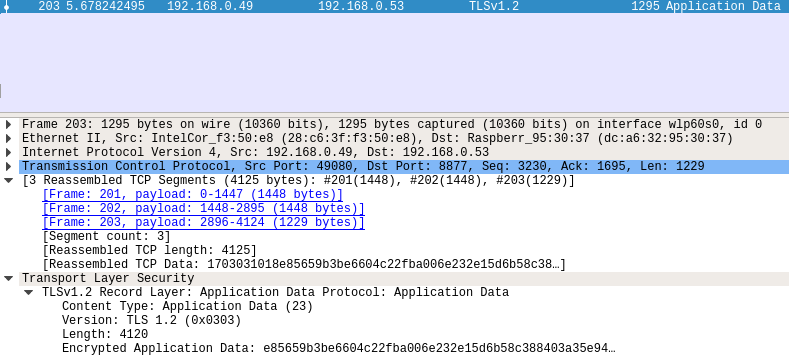
\includegraphics[scale=0.47]{./code/img/application_data_wolfSSL.png}
    \caption{Application data wolfSSL}
\end{figure}
\begin{figure}[H]
    \centering
    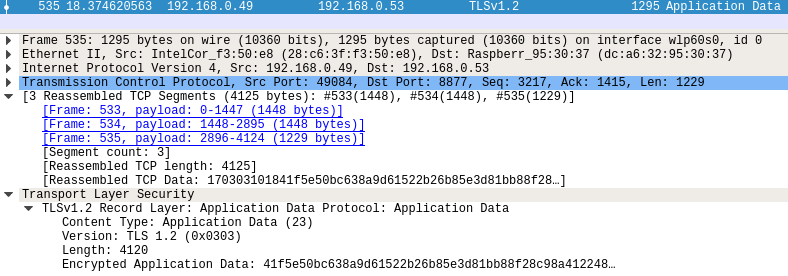
\includegraphics[scale=0.47]{./code/img/application_data_openSSL.png}
    \caption{Application data openSSL}
\end{figure}


\section{Conclusion}
WolfSSL is a beautiful very well done library. They have a forum where thousand of users report their problems and solutions, in which employees too are very active.

A problem of wolfSSL manual is the lack of some details in some sections, such as in the difference with openSSL and its self-promotion orientation.

I think that this thesis can be a good starter guide to get information about wolfSSL since it is difficult to find material from the non official channels.

%\vspace{5mm} %5mm vertical space
It is actively being used in a wide range of markets and products including the smart grid, IoT, industrial automation, connected home, M2M, auto industry, games, applications, databases, sensors, VoIP, routers, appliances, cloud services, and more; since wolfSSL is widely employed at a corporate level, there is a great lack of open source projects on the net.

%\vspace{5mm} %5mm vertical space
In the future I intend to carry on this research, also focusing on wolfSSL's other products, such as wolfSSH, wolfCrypt, etc.

\begin{thebibliography}{9}

\bibitem{WolfSSLRepo} 
Official WolfSSL repository
\\\url{https://www.github.com/wolfSSL/wolfssl}

\bibitem{WolfSSLmanual} 
Official WolfSSL manual
\\\url{https://www.wolfssl.com}

\bibitem{Book}
William Stallings, ''Cryptography and Network Security Principles and Practice, Global Edition-Pearson (2017)'',
ISBN: 978-1292158587

\bibitem{Book}
Rolf Oppliger, ''SSL and TLS: Theory and Practice'',
ISBN: 978-1596934474
\bibitem{BookEmbeddedSystems}
Wiley, ''Communicating Embedded Systems: Networks Applications'',
ISBN: 978-1848211445

\end{thebibliography}



\end{document}
